
\documentclass[8pt]{beamer}

\usepackage{amsmath,amssymb,amsfonts}
\usepackage{mathrsfs}
\usepackage{color,xcolor}
\usepackage{graphicx}
\usepackage{clock} % Use this package to insert a clock in the beamer.
\usepackage{textcomp}
\usepackage[T1]{fontenc}
\usepackage{epstopdf}
\mode<presentation>
{
  \usetheme{Madrid}
   % 可供选择的主题参见 beameruserguide.pdf, 第 146 页起
  % 无导航条的主题: Bergen, Boadilla, Madrid, Pittsburgh, Rochester;
  % 有树形导航条的主题: Antibes, JuanLesPins, Montpellier;
  % 有目录竖条的主题: Berkeley, PaloAlto, Goettingen, Marburg, Hannover;
  % 有圆点导航条的主题: Berlin, Dresden, Darmstadt, Frankfurt, Singapore, Szeged;
  % 有节与小节导航条的主题: Copenhagen, Luebeck, Malmoe, Warsaw
  %\setbeamertemplate{footline}{}
  \usecolortheme{sustech} %主题颜色
  \setbeamercovered{transparent}
  %
}
% beamer
\usefonttheme{professionalfonts}
\usepackage[UTF8,noindent]{ctex}
%\usepackage{CJK}
\usepackage{color}
\usepackage{xcolor}


\newcommand{\R}{\mathbb{R}}
%\newcommand{\C}{\mathbb{C}}
\renewcommand{\i}{\mathbf{i}}
\newcommand{\ii}{\mathbf{i}}
\renewcommand{\Re}{\mathrm{Re}\,}
\renewcommand{\Im}{\mathrm{Im}\,}
\newtheorem{alg}{算法}[section]
\newtheorem{lem}{引理}[section]
\newtheorem{them}{定理}[section]
\newtheorem{assumption}{Assumption}[section]
\newtheorem{remark}{}[section]
\newtheorem{deff}{定义}[section]
\newtheorem{question}{}[section]
%\newtheorem{example}{\bf }[section]

\newcommand{\eps}{\varepsilon}
\newcommand{\RR}{\mathcal{R}}




\newcounter{RomanNumber}
\newcommand{\MyRoman}[1]{\rm\setcounter{RomanNumber}{#1}\Roman{RomanNumber}}

\newcommand{\bL}{\mathbf{L}}
\newcommand{\bH}{\mathbf{H}}
\newcommand{\bW}{\mathbf{W}}
\newcommand{\bP}{\mathbf{P}}
\newcommand{\bQ}{\mathbf{Q}}
\newcommand{\bp}{\mathbf{p}}
\newcommand{\bq}{\mathbf{q}}
\newcommand{\uL}{u_{_{\rm L}}}
\newcommand{\vL}{v_{_{\rm L}}}
\newcommand{\tuL}{\tilde u_{_{\rm L}}}
\newcommand{\tvL}{\tilde v_{_{\rm L}}}
\newcommand{\fL}{f_{_{\rm L}}}
\newcommand{\gL}{g_{_{\rm L}}}
\newcommand{\bpL}{\bp_{_{\rm L}}}
\newcommand{\bqL}{\bq_{_{\rm L}}}
\newcommand{\tbpL}{\tilde{\bp}_{_{\rm L}}}
\newcommand{\tbqL}{\tilde{\bq}_{_{\rm L}}}
\newcommand{\tbpLf}{\tilde{\bp}_{_{\rm L,1}}}
\newcommand{\tbpLs}{\tilde{\bp}_{_{\rm L,2}}}
\newcommand{\tbqLf}{\tilde{\bq}_{_{\rm L,1}}}
\newcommand{\tbqLs}{\tilde{\bq}_{_{\rm L,2}}}
\newcommand{\bn}{\nu}
\newcommand{\bv}{\mathbf{v}}
\newcommand{\om}{\omega}
\newcommand{\pa}{\partial}
\newcommand{\la}{\langle}
\newcommand{\ra}{\rangle}
\newcommand{\lla}{\la{\hskip -2pt}\la}
\newcommand{\rra}{\ra{\hskip -2pt}\ra}
\newcommand{\jj}{\|{\hskip -0.8pt} |}
\newcommand{\al}{\alpha}
\newcommand{\ze}{\zeta}
\newcommand{\si}{\sigma}
\newcommand{\ep}{\varepsilon}
\newcommand{\na}{\nabla}
\newcommand{\vp}{\varphi}
\newcommand{\ga}{\gamma}
\newcommand{\Ga}{\Gamma}
\newcommand{\Om}{\Omega}
\newcommand{\de}{\delta}
\newcommand{\Th}{\Theta}
\newcommand{\De}{\Delta}
\newcommand{\Lam}{\Lambda}
\newcommand{\lam}{\lambda}
\newcommand{\tri}{\triangle}
\newcommand{\lj}{[{\hskip -2pt} [}
\newcommand{\rj}{]{\hskip -2pt} ]}
\newcommand{\bks}{\backslash}
%\newcommand{\diag}{\mathrm{diag}}
\newcommand{\diam}{\mathrm{diam}}
\newcommand{\osc}{\mathrm{osc}}
\newcommand{\meas}{\mathrm{meas}}
\newcommand{\dist}{\mathrm{dist}}

\newcommand{\mL}{\mathscr{L}}
\newcommand{\cT}{{\cal T}}
\newcommand{\cM}{{\cal M}}
\newcommand{\cE}{{\cal E}}
\newcommand{\cL}{{\cal L}}
\newcommand{\cF}{{\cal F}}
\newcommand{\cB}{{\cal B}}
\newcommand{\PML}{{\rm PML}}
\newcommand{\FEM}{{\rm FEM}}
\newcommand{\rd}{\,\mathrm{d}}

\renewcommand{\i}{\mathbf{i}}
\renewcommand{\v}{\mathbf{v}}
\renewcommand{\u}{\mathbf{u}}
\renewcommand{\r}{\mathbf{r}}
\newcommand{\gR}{{\mathbb{R}}}
\newcommand{\Z}{{\mathbb{Z}}}
\renewcommand{\C}{{\mathbb{C}}}

\renewcommand{\Re}{\mathrm{Re}\,}
\renewcommand{\Im}{\mathrm{Im}\,}
\renewcommand{\div}{\mathrm{div}}
\newcommand{\curl}{\mathrm{curl}}
\newcommand{\Curl}{\mathbf{curl}}
\newcommand{\pv}{\mathrm{P.V}}

\newcommand{\Np}{\mathcal{N}_p}
\newcommand{\Ns}{\mathcal{N}_s}
\newcommand{\Tp}{\mathcal{T}_p}
\newcommand{\Ts}{\mathcal{T}_s}
\newcommand{\Na}{\mathcal{N}_\alpha}
\newcommand{\Nb}{\mathcal{N}_\beta}
\newcommand{\Ta}{\mathcal{T}_\alpha}
\newcommand{\Tb}{\mathcal{T}_\beta}
\newcommand{\GG}{\mathcal{G}}

\newcommand{\N}{\mathbb{N}}
\newcommand{\D}{\mathbb{D}}
\newcommand{\T}{\mathbb{T}}
\newcommand{\A}{\mathbb{A}}
\newcommand{\B}{\mathbb{B}}
\renewcommand{\G}{\mathbb{G}}
\newcommand{\F}{\mathbb{F}}

\renewcommand{\U}{\mathbb{U}}
\newcommand{\W}{\mathbb{W}}
\newcommand{\V}{\mathbb{V}}
\newcommand{\J}{\mathbb{J}}
\newcommand{\Zg}{\mathbb{Z}}
\newcommand{\Gtheta}{\mathbb{\Theta}}
\newcommand{\Gphi}{\mathbb{\Phi}}

%%%%%%%%%%%%%%%%%%%%%%%%%%%%%%%%%%%%%%%%%%%%%%%%%%%%%%%%%%%%%%%%%%%%
\newcommand{\be}{\begin{eqnarray}}
\newcommand{\ee}{\end{eqnarray}}
\newcommand{\ben}{\begin{eqnarray*}}
\newcommand{\een}{\end{eqnarray*}}
\newcommand{\nn}{\nonumber}



\def\debproof{\noindent {\bf ¨¨.} }
\def\finproof{\hfill {\small $\Box$} \\}

\begin{document}

\title[博士论文答辩]{半空间中的弹性波反散射问题}

\author[周世奇]{答辩人:周世奇 \\ \vspace{0.3cm} 导师:陈志明~研究员}
\institute[ICMSEC AMSS CAS]{\scriptsize 中国科学院\\[0.2em]
	数学与系统科学研究院\\[0.2em]
	计算数学与科学工程计算研究所}
\date[2019年5月]{2019年5月15日}

%学校 logo
%\pgfdeclareimage[height=0.5cm]{ucas_logo}{ucas_logo.pdf}
%\logo{\pgfuseimage{ucas_logo}\hspace*{0.3cm}}

% 如果你想要在每一小节之前都显示一下目录, 则可把一下小段的注解号 "%" 删去
\AtBeginSection[]
{
	\begin{frame}<beamer>
	\frametitle{目录}
	%    \tableofcontents[currentsection,currentsubsection]
	\tableofcontents[currentsection]
\end{frame}
}
%\AtBeginSubsection[]
%{
%  \begin{frame}<beamer>
%    \frametitle{Outline}
%    \tableofcontents[currentsection,currentsubsection]
%  \end{frame}
%}

% 除掉以下命令的注解 "%" 后, 许多环境都会自动逐段显示
%\beamerdefaultoverlayspecification{<+->}

\begin{frame}
  \titlepage
\end{frame}

\begin{frame}
  \frametitle{目录}
  \setcounter{tocdepth}{1}
  \tableofcontents%[pausesections]
\end{frame}

\section{研究背景}

\begin{frame}
\frametitle{地震波勘探模型}
\begin{figure}

  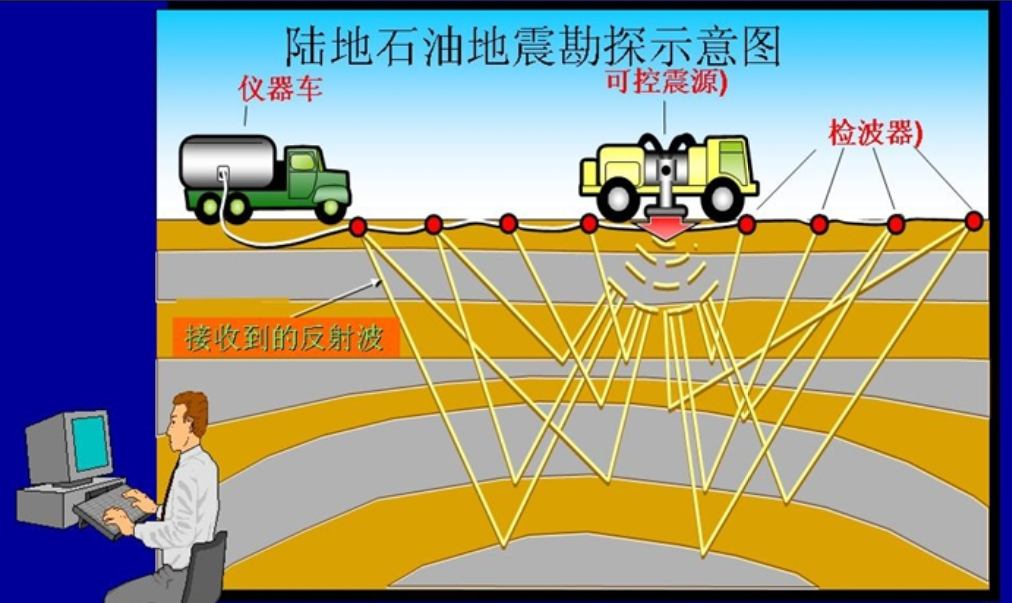
\includegraphics[width=10cm,height=5cm]{./figure/seismic.png}
  \caption{地震波勘探模型示意图}
\end{figure}
\end{frame}

\begin{frame}
\frametitle{抽象模型}
\begin{figure}
	\centering
	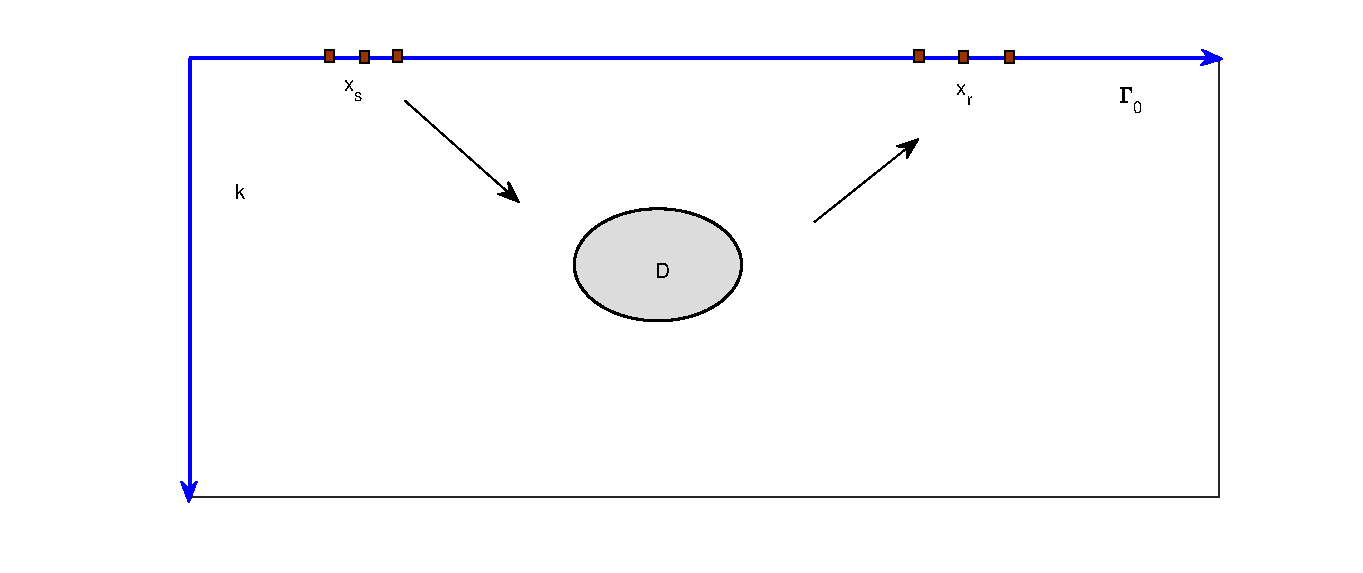
\includegraphics[width=10cm,height=5cm]{./figure/half_forward}
	\caption{半空间弹性波散射问题模型}
\end{figure}
\end{frame}

\begin{frame}
\frametitle{半空间弹性波散射问题}
假设在半空间中存在障碍物 $D\subset\R^2_+$,且为有界 Lipschitz 区域. 入射场是由位于$x_s$ 处的点源沿着极化方向 $q\in \R^2$ 激发,于是相对应的弹性波总场 $u_q(x,x_s)\in \C^2$ 满足如下半空间弹性波方程,
\ben\label{elastic_eq}
& &\nabla\cdot\sigma(u_q) + \omega^2u_q= -\delta_{x_s}(x)q \ \ \ \ \mbox{in }\R_+^2\bks \bar{D},\\
& &u_q=0 \ \ \mbox{on} \ \Ga_D  ,
\een
且弹性波总场在半空间表面满足自由表面边界条件即法向应力为零,
\ben
\sigma(u_q)\cdot e_2=0 \ \ \mbox{on} \ \Ga_0.
\een
其中应力张量 $\sigma(u)\in \C^{2\times2}$ 是2阶张量, 它与应变张量 $\ep(u)\in \C^{2\times2}$ 一起满足如下本构关系 (Hookes 定律),
\ben
& &\sigma(u) = 2\mu\ep(u) + \lambda\div u \mathbb{I}, \\
& &\ep(u)=\frac{1}{2}(\na u +(\na u)^T).
\een
为了简便,我们定义弹性波算子 :
\ben
& &\Delta_e u:=\nabla\cdot\sigma(u)=(\lambda+\mu)\nabla\div \ u+\mu\Delta u.
\een
\end{frame}

\begin{frame}
\frametitle{正问题与反问题}
	\begin{block}{正散射问题:}
		令$u^i_q(x,x_s)=\N(x,x_s)q$为入射场,其中$\N(x,y)$为半空间Neumann格林函数,然后求解散射场$u^s_q(x,x_s)=u_q(x,x_s)-u^i_q(x,x_s)$.
	\end{block}
\pause
$u_q^s(x,x_s)$ 满足如下方程,
\be
& &\Delta_e u_q^s(x,x_s)+ \omega^2u_q^s(x,x_s)= 0 \ \ \ \ \mbox{in }\R_+^2\bks \bar{D},\label{ep1}\\
& &u^s_q(x,x_s)=-\N(x,x_s)q \ \ \mbox{on} \ \Ga_D,\ \ \ \sigma(u_q^s(x,x_s))e_2=0 \ \ \mbox{on} \ \Ga_0.\label{ep2}
\ee
\pause
利用极限吸收原理来定义半空间弹性波散射问题的解.  令$u^s_{q,\ep}$ 是满足角频率为 $\om(1+\i\ep)$ 的半空间弹性波方程,即
\ben
& &\Delta_e u_{q,\ep}^s(x,x_s)+ \omega^2(1+\i\ep)^2 u_{q,\ep}^s(x,x_s)= 0 \ \  \mbox{in }\R_+^2\bks \bar{D},\label{p12}\\
& &u^s_{q,\ep}(x,x_s)=-\N(x,x_s)q \  \mbox{on} \ \  \Ga_D,\ \ \sigma(u_{q,\ep}^s(x,x_s))e_2=0 \ \  \mbox{on} \  \Ga_0 .\label{p22}
\een
于是, 方程(\ref{ep1})-(\ref{ep2}) 中的散射解 $u_q^s(x,x_s)$ 定义为 $u_{q,\ep}^s(x,x_s)$ 在 $\ep\to 0^+$ 时在空间$H^{1,-s}(\R^\bks\bar{D})$, $s>1/2$ 中的极限, 其中
\ben
H^{1,s}(\Om)=\{v(x): (1+|x|^2)^{s/2}v(x)\in L^{2,s}(\Om) , \ \  (1+|x|^2)^{s/2}\nabla v(x)\in L^{2,s}(\Om)   \}.
\een
\end{frame}

\begin{frame}
    \begin{block}{经典的正散射问题研究方法}
    	
    \end{block}
\end{frame}
\begin{frame}
	\begin{block}{反散射问题:}
		 通过在$\textcolor{blue}{\Gamma_0}$上接受到的\textcolor{red}{散射数据},构建算法来确定障碍物$D$ 的位置、大小和形状. 主要方法分为迭代法和直接成像法。
	\end{block}
\vspace{.5cm}
\pause
\begin{itemize}
	\item 迭代法是一种优化手段, 具体是将观察数据与初值参数构成目标函数, 然后将目标函数最小化的过程.  抽象为如下表达式:
	\ben
	\min_{\mathbf{m}} \ dist(\mathbf{d}^{obs},\mathbf{{L}}\mathbf{m}),
	\een
	其中 $\mathbf m$ 表示障碍物边界参数或是非均匀介质参数, $\mathbf{d}^{obs}$ 表示观测数据, $\mathbf{{L}}$ 表示正弹性波散射问题的解算子, $dist(\cdot,\cdot)$ 表示某种距离.
	
	\bigskip
	\pause
	\item 直接成像法的基本思想是构造一个指示性成像函数,代入观测数据后, 该函数值在远离障碍物边界时逐渐衰减; 在靠近边界时, 函数值趋于峰值.
	\begin{itemize}
		\item 线性采样法
		\item 分解法
		\item \textcolor{red}{逆时偏移算法}
	\end{itemize}
\end{itemize} 
\end{frame}

\begin{frame}
\frametitle{常见算法分类与介绍}
\begin{columns}
	
	\column{.45\textwidth}
	
	\begin{block}{直接成像法}
		\begin{itemize}
			\item 线性采样法(LSM),分解法(Factorization method),点源法(Point source method)
			\item MUSIC成像算法(MUltiple SIgnal Classification)
			\item 叠前深度偏移(Prestack depth migration),\textcolor{blue}{逆时偏移算法}
		\end{itemize}
		
	\end{block}
	\begin{block}{特点}
		可以直接成像,计算速度快,但较难给出定量的介质参数信息,且严格的数学理论并不完善
	\end{block}
	\column{.45\textwidth}
	
	\begin{block}{迭代法}
		\begin{itemize}
			\item 微分相似优化算法(Differential semblance optimization)
			\item 全波形反演(Full waveform inversion)
			\item 逐步线性化算法(Recursive linearization algorithm)
		\end{itemize}
	\end{block}
	\begin{block}{特点}
		可以得到定量信息,但是需要先验信息,计算耗时,收敛性分析困难
	\end{block}
\end{columns}
\begin{block}{逆时偏移算法(Reverse Time Migration)}
	基于波动方程反传播和时逆的想法,能够对复杂地质构造进行有效成像,被广泛应用,但是之前的理论分析需要
	\textcolor{red}{高频渐进假设}或者\textcolor{red}{几何光学近似}.
\end{block}
\end{frame}

\section{半空间弹性波 Green 函数}
\begin{frame}
\frametitle{Neumann Green 函数}
设源点$y\in\R^2_+$, 引入半空间弹性波Neumann零边界格林函数$\N(x,y)$, 对任意向量$q\in\R^2$, 其满足如下方程:
\ben
& & \Delta_e [\N(x;y)q] + \omega^2 [\N(x,y)q] = -\mathbf{\delta}_y(x) q \ \ \mbox{in }\R^2_+ , \label{eq_n1} \\
& & \sigma(\N(x,y)q)e_2 = 0 \ \ \mbox{on } \Gamma_0, \label{eq_n2}
\een
${\delta}_y(x)$代表位于点y的Dirac源. 对$\N(x,y)$关于$x_1$变量作Fourier变换得到
\ben
\hat \N(\xi,x_2;y_2)= \int_\R\N(x_1,x_2;y) e^{-\i (x_1-y_1)\xi} dx_1,\ \ \forall \xi\in\C.
\een
为了利用基本解$\G(x,y)$在 $x=y$ 处的奇性,我们令
\ben
\N_c(x,y)=\N(x,y)-(\G(x,y)-\G(x,y')),
\een
其中$y'=(y_1,-y_2)$ 为y关于$x_1$轴的镜像点. 利用常系数常微分方程组的标准解法,我们得到
\ben\label{NGT}
\hat \N_c(\xi,x_2;y_2) =  \frac{\i}{\omega^2\delta(\xi)}\sum_{\alpha,\beta=p,s}\mathbb{A}_{\al\beta}(\xi)e^{\i(\mu_\al x_2+\mu_{\beta} y_2)}, 
\een
\end{frame}

\begin{frame}
其中 $\varphi(\xi)=k_s^2-2\xi^2$, $\delta(\xi)=\varphi(\xi)^2+4\xi^2\mu_s\mu_p $, $\mu_\alpha=(k_\alpha^2-\xi^2)^{1/2}$,$\alpha=s,p$, $k_p=\omega/\sqrt{\lam+2\mu}, k_s=\omega/\sqrt{\mu}$为p波和s波的波数, 及 

\ben
&&{\mathbb{A}_{ss}(\xi)} =
\left( \begin{array}{ll}
	\varphi^2\mu_s & -4\xi^3\mu_s\mu_p \\
	-\xi\varphi^2  & 4\xi^4\mu_p
\end{array} \right),\ \ 
{\mathbb{A}_{sp}(\xi)} =
\left( \begin{array}{ll}
	2\xi^2\varphi\mu_s & -2\xi\varphi\mu_s\mu_p \\
	-2\xi^3\varphi  & 2\xi^2\varphi\mu_p
\end{array} \right),\\ 
\\
\\
&&
{\mathbb{A}_{ps}(\xi)} =
\left( \begin{array}{ll}
	2\xi^2\varphi\mu_s & 2\xi^3\varphi \\
	2\xi\varphi\mu_s\mu_p  & 2\xi^2\varphi\mu_p
\end{array} \right),\ \ 
{\mathbb{A}_{pp}(\xi)} =
\left( \begin{array}{ll}
	4\xi^4\mu_s & \xi\varphi^2 \\
	4\xi^3\mu_s\mu_p  & \varphi^2\mu_p
\end{array} \right).
\een
\pause
\begin{remark}
	我们假设对于任意的$z\in \mathbb{C}\backslash\{0\}$, $z^{1/2}$是多值函数$\sqrt{z}$ 的如下解析分支:$\Im(z^{1/2})\geq 0$,这对应于在复平面取右半实轴为割支线. 则对于$z=z_1+\mathbf{i}z_2$, $z_1,z_2\in\R$,
	\ben \label{convention_1}
	z^{1/2}={\rm sgn}(z_2)\sqrt{\frac{|z|+z_1}{2}}+\i\sqrt{\frac{|z|-z_1}{2}},\ \ \forall z\in\C\backslash\bar{\R}_+.
	\een
	当$z$位于右半实轴的上沿或是下沿时,取$z^{1/2}$为$\ep\rightarrow0^+$ 时$(z+\i\ep)^{1/2}$ 或是 $(z-\i\ep)^{1/2}$的极限即可. 
\end{remark}

\end{frame}

\begin{frame}
	\begin{lem} \label{rayleigh}
		Rayleigh方程 $\delta(\xi) = 0$在复平面$\C$中有且仅有两个根且记为 $\pm k_R$, 其中$k_R$满足$k_R>k_s$. 
	\end{lem}
由此可得 $\hat \N(\xi,x_2;y_2)$ 在实轴上存在极点,不能直接对其进行 Fourier 逆变换。
\pause
\begin{lem}\label{complex_rayleigh}
	记$\delta_{\om(1+\i\ep)}(\xi)$为将$\delta(\xi)$中的$k_p,k_s$替换成$k_s(1+\i\ep),  k_p(1+\i\ep)$后相应的复Rayleigh方程. 复Rayleigh方程 在$\C\bks{\bar{\Om}}$中有且仅有两个根且为$\pm k_R(1+\i\ep)$.  其中集合$\Om$为
	\ben\label{set:Om}
	\Omega := \{\xi_1+\i\xi_2 \in \mathbb{C} \ | \ k_p^2\ep<\xi_1\xi_2<k_s^2\ep \ , \  \ \xi_2/\xi_1>\ep\}.
	\een
\end{lem}

记 $\mathbb{N}_{\omega(1+\i\ep)}(x,y)$ 为将实圆频率$\omega$ 替换为复圆频率$\om(1+\i\ep)$后相应方程的Green函数. 由上述引理可知 $\hat\N_{\omega(1+\i\ep)}(\xi,x_2;y_2)$ 在实轴上没有极点, 可以对其直接进行逆Fourier变换.  于是,半空间弹性波 Neumann Green函数 $\mathbb{N}(x,y)$ 可以利用极限吸收原理得到,即为
\ben
\N(x,y)&=&\lim_{\ep\to 0^+} \N_{\om(1+\i\ep)}(x,y)\\ \label{NGT1}
&=&\lim_{\ep\to 0^+}\frac{1}{2\pi}\int_\R\hat \N_{\om(1+\i\ep)}(\xi,x_2;y_2) e^{\i(x_1-y_1)\xi} d\xi.
\een
\end{frame}

\begin{frame}
\frametitle{割支线示意图}
\begin{figure}
	\centering
	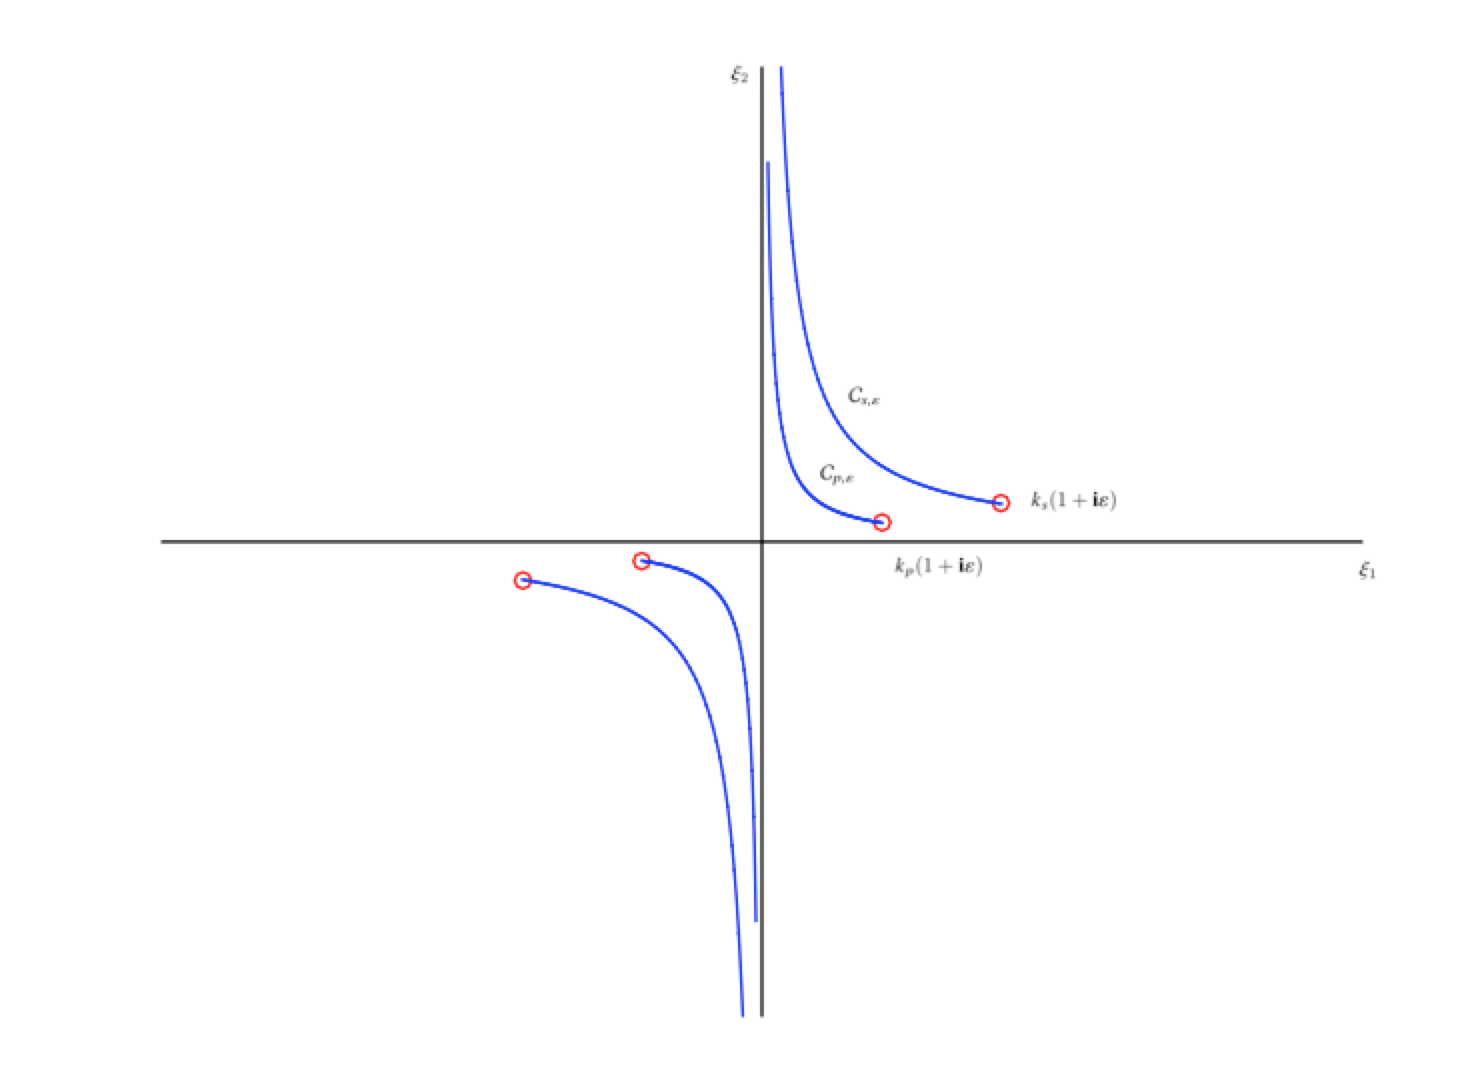
\includegraphics[width=10cm,height=5cm]{./figure/cut_plot}
	\caption{$\mu_p(\xi),\mu_s(\xi)$的割支线}
\end{figure}
\end{frame}
\begin{frame}
	\begin{lem}\label{cauchy_pv}
		令 $a,b\in\R,\  a<b$, 且 $t_0\in (a,b)$. 如果 $\gamma$ 在$[a,b]$上 H\"older 连续, 即存在常数 $\alpha\in (0,1]$ 及 $C>0$ 对于任意 $s,t\in [a,b]$, $|\gamma(s)-\gamma(t)|\le C|s-t|^\alpha$, 于是有
		\ben
		\lim_{z\to t_0,\pm\Im z>0}\int^b_a\frac{\gamma(t)}{t-z}dt={\rm p.v.}\int^b_a\frac{\gamma(t)}{t-t_0}dt\pm\pi\i\ga(t_0),
		\een
		其中 ${\rm p.v.}\int^b_a$ 表示积分的Cauchy主值. 
	\end{lem}
\bigskip

	由以上引理,我们就可以得到如下 Neumann Green 函数的表达式:
	\ben\label{NGT2}
	\N(x,y)&=&\frac{1}{2\pi}\,{\rm p.v.}\int_{\R}\hat \N(\xi,x_2;y_2) e^{\i(x_1-y_1)\xi} d\xi\\
	& &-\frac{1}{2\omega^2}
	\left[\sum_{\alpha,\beta=p,s}\frac{\mathbb{A}_{\al\beta}(\xi)}{\de'(\xi)}e^{\i(\mu_\al x_2+\mu_\beta y_2)+\i(x_1-y_1)\xi}\right]^{k_R}_{-k_R},\ \ \forall x,y\in\R^2_+,
	\een
	这里 $[f(\xi)]^b_a:=f(b)-f(a)$ . 
\end{frame}

\begin{frame}
	对于 $x_s\in\Ga_0$ 时的情况, 我们可以定义对应的 Neumann Green 函数 $\N(x,x_s),x\in\R^2_+$ 为 $\N(x,y)$ 在 $y\in\R^2_+,  \  y\to x_s$ 时的极限.  可以将 $\N(x,y)$ 简化为:
	\ben
	\hat
	\N(\xi,0;y_2)= 
	:=\frac{1}{\delta(\xi)}(\Np(\xi)e^{\i\mu_p y_2}+\Ns(\xi)e^{\i\mu_s y_2}). \label{d2}
	\een

	\begin{lem}\label{lem:2.3} 令 $x\in\Ga_0 \ , y\in \R^2_+$ 以及 $\phi\in (-\pi/2,\pi/2)$ 且 $y_2=|x-y|\cos\phi \ $ ,
		$x_1-y_1=|x-y|\sin\phi$ .  假设 $x_1\not= y_1$, 于是可以得到
		\ben\label{NGT3}
		\N(x,y)&=&\frac{1}{2\pi}\sum_{\al=p,s}\int_L\mathbb{N}_0^\al(t)\cos(t+\phi)e^{\i\lam_\al\cos t}dt \\
		\nn
		& & \pm\i
		\left[\sum_{\al=p,s}\frac{\Na(\xi)}{\de'(\xi)}e^{\i\mu_\al y_2+\i(x_1-y_1)\xi}\right]_{\xi=\pm k_R},\label{h3}
		\een
		其中 $\lam_\al=k_\al|x-y|, \ \al=s,p $, $L$ 为复平面中的积分路径即 从 $-\pi/2+\i\infty$ 到 $-\pi/2$, $-\pi/2$ 再到 $\pi/2$, 接着从 $\pi/2$ 到 $\pi/2-\i\infty$ 的折线 , 这里符号 $\pm$ 取决于 ${\rm sgn}(x_1-y_1)=\pm 1$, 且定义表达式:
		\ben\label{h2}
		\mathbb{N}_{0}^\al(t)=k_\al\,\frac{\Na(k_\al\sin(t+\phi))}{\de(k_\al(\sin(t+\phi))}, \ \ \ \al=s,p.
		\een
	\end{lem}
	
\end{frame}
\begin{frame}
\frametitle{积分路径示意图}
\begin{figure}
	\centering
	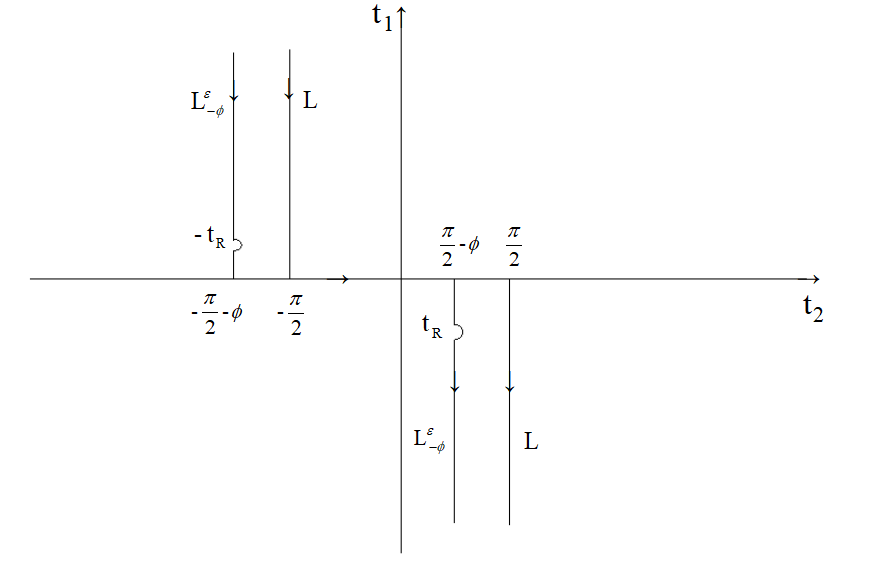
\includegraphics[width=10cm,height=5cm]{./figure/transformation4.png}
	\caption{积分路径示意图}
\end{figure}
\end{frame}

\begin{frame}
\frametitle{$\N(x,y)$的渐近估计}
\begin{lem}[Van der corput]\label{lem:2.5}
	令 $\lam\ge 1$, 假设$f\in C[-\pi/2,\pi/2]$ 且其导函数绝对可积.  于是对任意区间 $(a,b)\subset (-\pi/2,\pi/2)$, 可以得到
	\ben\label{c1}
	\left|\int_a^bf(t)e^{\i\lam\cos t}dt\right| 
	\leq C\lam^{-1/2}\left(|f(0)|+\int_a^b|f'(t)|dt\right),
	\een
	这里常数 $C$ 与 $a,b,\lam$ 及被积函数 $f$ 无关.  
	此外, 令 $\kappa\in (0,1)$ 以及 $\phi\in (-\pi/2,\pi/2)$ 满足条件 $|\phi|\geq\phi^*>\arcsin \kappa:=\phi_\kappa$ , 可以得到
	\ben\label{c3}
	\left|\int_{-\frac\pi 2}^{\frac\pi 2}f(t)(\kappa^2-\sin^2(t+\phi))^{-1/2}e^{\i\lam\cos t}dt\right|  
	\leq C\lam^{-1/2}\left(|f(0)|+\int_{-\frac\pi 2}^{\frac \pi2}|f'(t)|dt\right),
	\een
	这里常数 $C$ 只与 $\phi^*$ 和 $\kappa$ 有关. 
\end{lem}
\pause
\begin{them}\label{es_NGT}
	假定 $x\in\Gamma_0$, $y\in\R_+^2$ 且满足 $|x_1-y_1|/|x-y|\ge(1+\kappa)/2$ 及 $k_sy_2\ge 1$ . 存在只与 $\kappa$ 有关的常数 $C$ , 使得如下估计成立:
	\ben
	|\N(x,y)|+k_s^{-1}|\na_y\N(x,y)|\leq \frac{C}{\mu}\left(\frac{k_sy_2}{(k_s|x-y|)^{3/2}}+e^{-\sqrt{k_R^2-k_s^2}y_2}\right).
	\een
\end{them}
\end{frame}




\begin{frame}
\frametitle{Dirichlet Green 函数}
设源点$y\in\R^2_+$, 引入半空间弹性波Dirichlet零边界格林函数$\D(x,y)$, 对任意向量$q\in\R^2$, 其满足如下方程:
\ben
& & \De_e [\D(x,y)q] + \omega^2 [\D(x,y)q] = -\mathbf{\de}_y(x)q \ \ \mbox{in } \R^2_+ , \label{eq_d1} \\
& &  \D(x,y)q = 0 \ \ \mbox{on } \Ga_0. \label{eq_d2}
\een
类似地,对 $\D(x,y)$关于 $x_1$ 做Fourier变换得到 $\hat \D(\xi,x_2;y_2)$,
\ben
\hat \D(\xi,x_2;y_2) &=& \hat \G(\xi,x_2;y_2)  -\hat \G(\xi,x_2;-y_2) \\
& &+ \frac{\i}{\omega^2 \gamma(\xi)}\sum_{\al,\beta=s,p}\mathbb{B}_{\al\beta}(\xi)e^{\i(x_2\mu_\alpha+y_2\mu_\beta)},\label{DGT}
\een
这里有
\ben
& &\gamma(\xi)=\xi^2+\mu_s\mu_p , \ \mathbb{B}_{sp}(\xi)=-\mathbb{B}_{ss}(\xi), \ \mathbb{B}_{ps}(\xi)=-\mathbb{B}_{pp}(\xi),
\\
\\
& &{\mathbb{B}_{ss}(\xi)} =
\left( \begin{array}{ll}
	\xi^2\mu_s & -\xi\mu_s\mu_p \\
	-\xi^3  & \xi^2\mu_p
\end{array} \right),\ \ \ \ \ \
{\mathbb{B}_{pp}(\xi)} =
\left( \begin{array}{ll}
	\xi^2\mu_s & \xi^3 \\
	\xi\mu_s\mu_p  & \xi^2\mu_p
\end{array} \right).
\een
\end{frame}

\begin{frame}
特别地, 我们针对 $x\in\Ga_0, y\in\R^2_+$, 定义 $\T_D(x,y)\in\C^{2\times 2}$ 为 Dirichlet Green 函数 $\D(x,y)$ 在 $e_2$ 方向的关于变量 $x_2$ 的应力向量 , 记为
\ben
\T_D(x,y)q=\sigma(\D(x,y)q)e_2, \forall q\in\R^2.
\een 
可以得到
\ben\label{DGT2}
\T_D(x,y)=\frac{1}{2\pi}\int_{\R}\hat \T_D(\xi,0;y_2) e^{\i(x_1-y_1)\xi}d\xi,\ \ \ \ \forall x\in\Ga_0,
\een
其中 
\ben\hspace{-1cm} 
\hat\T_D(\xi,0;y_2)&=&\frac 1{\gamma(\xi)}\left[\left(   \begin{array}{cc}
	\xi^2 & -\xi\mu_p \\
	-\xi\mu_s & \mu_p\mu_s
\end{array} \right)e^{\i\mu_p y_2}+
\left(   \begin{array}{cc}
	\mu_s\mu_p & \xi\mu_p \\
	\xi\mu_s & \xi^2
\end{array}\right)e^{\i\mu_s y_2}\right]\nonumber\\
\\
&:=&\Tp(\xi)e^{\i\mu_p y_2}+\Ts(\xi)e^{\i\mu_s y_2}.\label{d1}
\een
\begin{them}\label{es_DGT}
	令 $x\in\Gamma_0$, $y\in\R_+^2$ 满足 $|x_1-y_1|/|x-y|\ge (1+\kappa)/2$ 和 $k_s y_2\ge 1$ .  存在只与 $\kappa:=k_s/k_p$ 有关的常数 $C$ 成立如下估计
	\ben
	|\T_D(x,y)|+k_s^{-1}|\na_y\T_D(x,y)|\leq C\frac{k_s^2 y_2}{(k_s|x-y|)^{3/2}}.
	\een
\end{them}
\end{frame}

\begin{frame}
	\frametitle{半空间弹性波正散射问题的适定性}
	\begin{them}\label{thm:4.2}
	(1)	假设 $g\in H^{1/2}(\Ga_D)$,
		\be\label{e11}
			\Delta_e u_1 + \omega^2 u_1=0 \ \  \mbox{\rm in } \R^2_+\bks \bar{D},\ \ 
		 u_1= g \ \ \mbox{\rm on } \Ga_D,\ \ \sigma(u_1)e_2=0 \ \ \mbox{\rm on } \Ga_0, \label{e12}
		\ee
		半空间散射问题 (\ref{e11})
		存在唯一的散射解 $u\in H^{1}_{\rm loc}(\R^2_+ \backslash \bar D)$. 此外, 对于任意有界区域 $\mathcal O\subset \R^2_+\bks\bar D$ 存在常数 $C>0$ 成立如下估计:
		\ben
		\|u\|_{H^{1}(\mathcal O)}\le C\|g\|_{H^{1/2}(\Ga_D)}.
		\een
	(2)	假设$u_2$是如下全空间散射问题的散射解,
		\be
			\Delta_e u_2 + \omega^2 u_2=0 \ \  \mbox{\rm in }\R^2\bks \bar{D},\ 
			u_2 = g \ \ \mbox{\rm on } \Ga_D. \label{e22}
		\ee
		于是存在仅依赖于 $\kappa$ 而与 $k_s, h,d_D$ 都无关的常数 $C>0$, 成立如下估计,
		\ben
		& &\|\sigma(u_1-u_2)\nu\|_{H^{-1/2}(\Gamma_D)}\\
		&\le&\frac{C}{\mu}(1+\|T_1\|)(1+\|T_2\|)(1+k_s d_D)^2(k_sh)^{-1/2}\|g\|_{ H^{1/2}(\Ga_D)}.
		\een
		这里 $T_1, \ T_2 \ :H^{1/2}(\Ga_D)\to H^{-1/2}(\Ga_D)$  是弹性波散射问题 (\ref{e11}) 和 (\ref{e22}) 相应的 Dirichlet-to-Neumann 算子.  $\|T_1\|, \|T_2\|$ 表示相应的算子范数. 
	\end{them}
\end{frame}
\section{半空间弹性波反散射问题的直接成像法}

\begin{frame}
\frametitle{反散射问题}
\begin{columns}
\begin{column}{.5\textwidth}

\begin{tiny}
\begin{eqnarray*}
\left\{
\begin{array}{lll}
\Delta_e u_q^s(x,x_s) + \omega^2u_q^s(x,x_s)= -\delta_{x_s}(x)q \ \ \ \ &in&\R_+^2\bks \bar{D}\\
u_q^s(x,x_s)=-\N(x,x_s)q \ \  \ \ \ \ \ \ \ &on& \ \Ga_D  \ \ \\
\sigma(u_q^s(x,x_s))\cdot e_2=0 \ \ &on& \ \Ga_0
\end{array}
\right.
\end{eqnarray*}
\end{tiny}
\end{column}

\begin{column}{.35\textwidth}
\begin{figure}
  \centering
  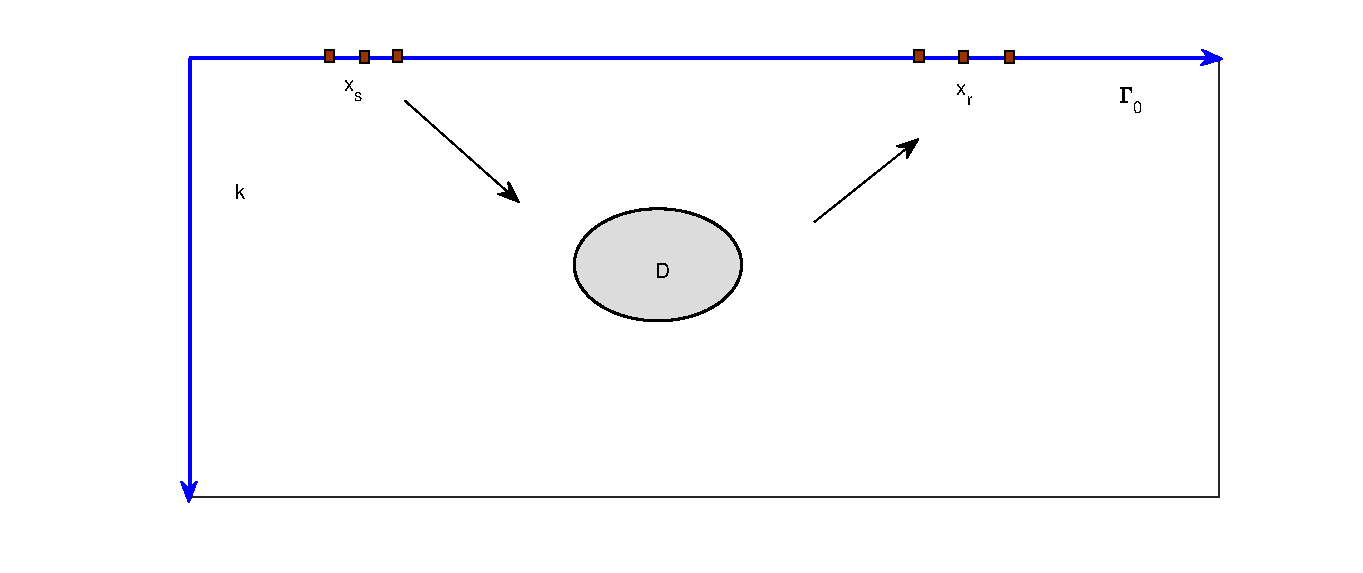
\includegraphics[width=4cm,height=2.5cm]{./figure/half_forward}
\end{figure}
\end{column}
\end{columns}
\begin{block}{发射器与接收器设置}
假设在 $\Ga_0^d=\{(x_1,x_2)^T\in\Ga_0: x_1\in (-d,d)\}$ 内均匀分布着 $N_s$ 个发射器, 位于 $x_s, \ s= 1,...,N_s$, 及分布着 $N_r$ 个接收器, 位于 $x_r, \ r=1,...,N_r$. 假设散射数据 $u_q^s(x_r,x_s)$ 为在 $x_r$ 处接收, 由位于 $x_s$ 处的点源沿着极化方向 $q=e_1, e_2$ 激发.
\end{block}
\begin{block}{采样区域设置}
令 $\Omega$ 为成像函数的采样区域,假设障碍物 $D\subset \Om$. 定义 $h=\dist(\Omega,\Gamma_0)$ 是 $\Omega$ 与 $\Gamma_0$ 的距离. 此外,我们假设存在常数 $0<c_1<1,c_2>0$ 使得下述条件成立:
\ben\label{d0}
|x_1|\leq c_1 d , \ \ \ \ \ \ \ \ |x-y|\leq c_2 h ,\ \ \ \ \forall x,y \in \Omega.
\een
\end{block}
\end{frame}


\begin{frame}
\frametitle{逆时偏移算法}
\begin{alg}
	$1^\circ$ 反传: 将观测数据 $\overline{u_q^s(x_r,x_s)}$反传到半空间中形成反传波 $v_q(x,x_s)$, 反传波是如下半空间弹性波散射问题的解
\ben
& &\Delta_e v_q(x,x_s) + \omega^2 v_q(x,x_s) =0 \ \ \ \ \ \mbox{\rm in } \ \ \R^2_+, \\
& &v_q(x,x_s)=\frac{|\Ga_0^d|}{N_r}\sum_{r=1}^{N_r}\overline{u_q^s(x_r,x_s)}\delta_{x_r}(x) \ \ \mbox{\rm on }  \ \ \Ga_d.
\een

$2^\circ$ 互相关: 对于任意 $q\in\R^2$,令入射波 $u^i_q$ 为如下半空间弹性波方程的解,
\ben
& &\Delta_e u_q^i(x,x_s) + \omega^2 u_q^i(x,x_s) =0 \ \ \mbox{\rm in } \ \ \R^2_+,\ \ \\ & &u^i_q(x,x_s)=q\de_{x_s}(x)\ \ \mbox{on } \ \ \Ga_d.
\een

对于任意 $z\in\Om$, 计算成像函数:
\ben\label{cor1} 
I_d(z)=\Im\sum_{q=e_1,e_2}\left\{\frac{|\Gamma_0^d|}{N_s}\sum^{N_s}_{s=1} u^i_q(z,x_s)\cdot v_q(z,x_s)\right\}. 
\een
\end{alg}
\end{frame}
\begin{frame}
于是, 由 Green 表示公式可以得到:
	\ben
	& &u^i_q(x,x_s)=\textcolor{red}{\T_D(x_s,x)}^Tq, \\
	& &v_q(x,x_s)\cdot e_j=\frac{|\Ga_0^d|}{N_r}\sum_{r=1}^{N_r}\textcolor{red}{\T_D(x_r,x)}e_j\cdot\overline{u_q^s(x_r,x_s)}.
	\een 
从而我们得到如下成像函数:
\begin{block}{离散型成像函数}
\ben\label{cor}
I_d(z)=\Im\sum_{q=e_1,e_2}\left\{\frac{|\Gamma_0^d|^2}{N_sN_r}\sum^{N_s}_{s=1}\sum^{N_r}_{r=1}
[\T_D(x_s,z)^Tq]\cdot[\T_D(x_r,z)^T\overline{u^s_q(x_r,x_s)}]\right\}.
\een
\end{block}
上面的成像函数是离散形式的, 可以直接用于数值计算. 为了理论分析, 我们令 $N_s,N_r\to\infty$, 于是离散形式的成像函数可以看成是采用数值积分对如下连续形式的成像函数的一种积分逼近:
\begin{block}{连续型成像函数}
\ben
\hat{I}_d(z)=\Im\sum_{q=e_1,e_2}\int_{\Gamma_0^d}\int_{\Gamma_0^d}\,
[\T_D(x_s,z)^Tq]\cdot[\T_D(x_r,z)^T\overline{u^s_q(x_r,x_s)}]\,ds(x_r)ds(x_s).\label{cor2}
\een
\end{block}
\end{frame}






\begin{frame}
\frametitle{逆时偏移算法:数学理论框架}
\begin{small}
	\begin{block}{全空间声波、电磁波及弹性波:}
		\begin{enumerate}
			\item Chen J, Chen Z, Huang G. {\it Reverse time migration for extended obstacles: acoustic waves [J]}. Inverse Problems. 2013, 29(8):645-648
			\item Chen J, Chen Z, Huang G. {\it Reverse time migration for extended obstacles: Electromagnetic waves[J]}. Scientia Sinica, 2015, 29(8):085005.
			\item Chen Z, Huang G. {\it Reverse time migration for extended obstacles: Elastic waves (in Chinese)[J]}. Science China Mathematics, 2015, 45(8):1103-1114.
		\end{enumerate}
	\end{block}
	\begin{block}{平板声波闭波导:}
		\begin{enumerate}
			\item Chen Z M, Huang G H. {\it Reverse time migration for reconstructing extended obstacles in planar acoustic waveguides[J]}. Science China Mathematics, 2015, 58(9):1811-1834.
		\end{enumerate}
	\end{block}
	
	\begin{block}{声波半空间:}
		\begin{enumerate}
			\item Chen Z, Huang G. {\it Reverse time migration for reconstructing extended obstacles in the half space[J].} Inverse Problems, 2015, 31(5):055007 (19pp).
		\end{enumerate}
	\end{block}
	
	\begin{block}{扩展:无相位成像算法}
		\begin{enumerate}
			\item Chen Z, Huang G. {\it Phaseless Imaging by Reverse Time Migration: Acoustic Waves[J]. } Numerical Mathematics Theory Methods and Applications, 2017, 10(1):1-21.
			%  \item Chen Z, Huang G. {\it A Direct Imaging Method for Electromagnetic Scattering Data without Phase Information[J]. }Siam Journal on Imaging Sciences, 2016, 9(3).
			%  \item Chen Z, Fang S, Huang G. {\it A Direct Imaging Method for the Half-Space Inverse Scattering Problem with Phaseless Data[J].} Inverse Problems and Imaging, 2017, 11(5).
		\end{enumerate}
	\end{block}
\end{small}

\end{frame}

\begin{frame}
\frametitle{点扩散函数(\textcolor{red}{P}oint \textcolor{red}{S}pread \textcolor{red}{F}unction)}
点扩散函数是用来对点源成像的函数,且弹性波情形下的PSF是一个 $2\times2$ 的矩阵. 假设在半空间的表面 $\Ga_0^d$ 上接收到位于 $y$ 处的点源场. 于是我们将有限孔径点扩散函数 $\J_d(x,y)$, $x,y\in\R^2_+$ 定义为将数据 $\overline{\N(x,y)}\chi_{(-d,d)}$ 反传入半空间中, 这里 $\chi_{(-d,d)}$ 为区间 $(-d,d)$ 上的特征函数. 
\ben
& &\De_e[\J_d(x,y)e_j]+\om^2[\J_d(x,y)e_j]=0\ \ \mbox{in }\R^2_+,\\
& &\J_d(x,y)e_j=[\overline{\N(x,y)}e_j]\chi_{(-d,d)}\ \ \mbox{on }\Ga_0.
\een
利用弹性波的积分表示公式, 我们有,对于任意的 $z,y\in\R^2_+$ ,
\ben
[\J_d(z,y)]_{ij}&=&e_i\cdot[\J_d(z,y)e_j]\\
&=&\int_{\Ga_0^d}\T_D(x,z)e_i\cdot\overline{\N(x,y)}e_jds(x),\ \ i,j=1,2.
\een
进一步利用矩阵表达, 可以简化为
\ben\label{jd}
\J_d(z,y)=\int_{\Ga_0^d}\T_D(x,z)^T\overline{\N(x,y)}ds(x).
\een
\end{frame}

\begin{frame}
\frametitle{数值实验: PSF}
从以下两张图可以看出 $\J_d(z,y)$ 的虚部也与弹性波基本解 $\Im\G(z,y)$ 的虚部有相似的函数特性.
\begin{columns}
	
	\column{.45\textwidth}
	\begin{figure}[h]
		\centering
		\includegraphics[width=\textwidth]{./graphic/green_om_2_lm_5_mu_25_im.eps}
		\caption{$\Im(\G(z,y))$ for $y=(0,8)^T$, $\omega=2\pi$, 其中 $\Im [\G(z,y)]_{ij}$ 对应于上面位置为$(i,j)$的子图.}
	\end{figure}
	\column{.45\textwidth}
	\begin{figure}[h]
		\centering
		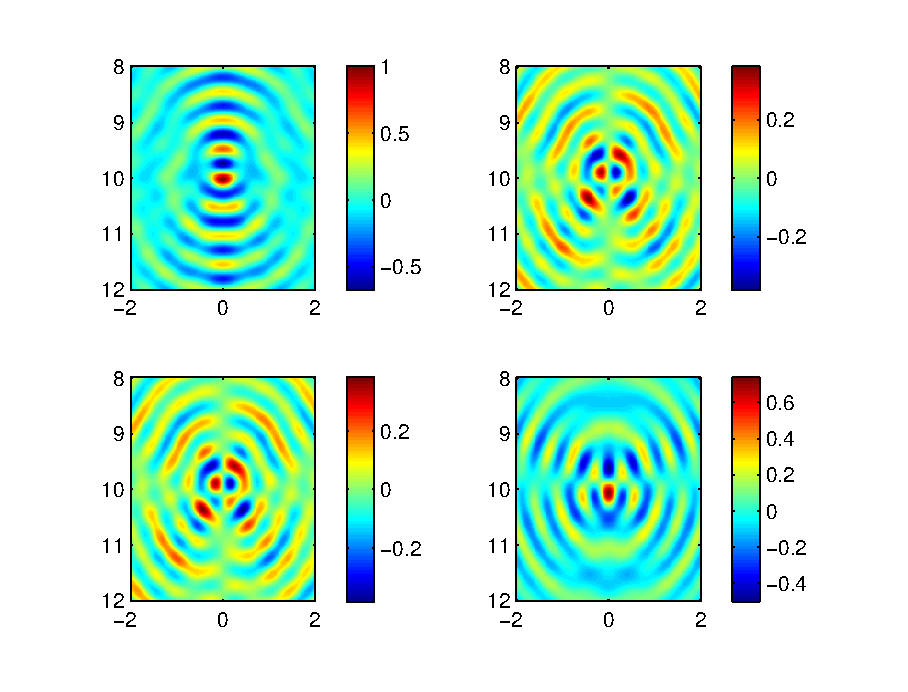
\includegraphics[width=\textwidth]{./graphic/psf_om_2_lm_5_mu_25_im.eps}
		\caption{$-\Im(\J_d(z,y))$, $y=(0,8)^T$, $\omega=2\pi$, $d=100$, $-\Im [\J_d(z,y)]_{ij}$ 对应位置$(i,j)$的子图.}
	\end{figure}
\end{columns}
\end{frame}

\begin{frame}
\frametitle{PSF的性质}
由 $\N(x,y)$及 $\T_D(x,y)$ 在无穷远处的渐近行为可知, 当 $d\to\infty$时, $\J_d(z,y)$ 收敛. 称$\lim\limits_{d\to\infty}\J_d(z,y)$为半空间弹性波点扩散函数 $\J(x,y)\in \C^{2\times 2}$, $x,y\in\R^2_+$, 即为
\ben\label{j}
\J(z,y)=\int_{\Ga_0}\T_D(x,z)^T\overline{\N(x,y)}ds(x)
\een
\begin{lem} \label{error_jd}
	假设 $k_s h\geq 1$ 和 $d\gg h$ . 对于任意 $z,y\in\Omega$ , 我们有
	\ben
	& &|\J(z,y)-\J_d(z,y)|+k_s^{-1}|\nabla_y(\J(z,y)-\J_d(z,y))| \\
	&\leq&\frac{C}{\mu} \left[\left(\frac{h}{d}\right)^{2}+(k_s h)^{1/2}e^{-k_s h\sqrt{\kappa_R^2-1}}\left(\frac{h}{d}\right)^{1/2}\right],
	\een
	这里常数 $C$ 只依赖于 $\kappa$ .
\end{lem}
由以上引理可知,当$d\gg h$ 时,我们只需分析 $\J(z,y)$ 的性质.
\end{frame}

\begin{frame}
	利用极限吸收原理, 我们得到
	\ben
	\J(z,y)=\lim_{\ep\to 0^+}\int_{\Ga_0} \T_D^{\,\omega(1+\i\ep)}(x,z)^T\,
	\overline{\N_{\om(1+\i\ep)}(x,y)}ds(x),
	\een
	这里 $\T_D^{\,\omega(1+\i\ep)}(x,z)q=\sigma(\D_{\om(1+\i\omega)}(x,z)q)e_2,\forall q\in\R^2$.
	利用 Parserval 等式, 我们可以得到
	\be
	\J(z,y)&=&\frac{1}{2\pi}\sum_{\al,\beta=p,s}{\rm p.v.}\int_{\R}\frac{{\Ta}(\xi)^T \overline{\Nb(\xi)}}{\overline{\delta(\xi)}} e^{\i (\mu_\alpha z_2-\overline{\mu}_\beta y_2)+\i(y_1-z_1)\xi} d\xi \nn \\
	& &-\frac\i 2\sum_{\al,\beta=p,s}\left[\frac{{\Ta}(\xi)^T \overline{\Nb(\xi)}}{\overline{\delta'(\xi)}} e^{\i (\mu_\alpha z_2-\overline{\mu}_\beta y_2)+\i(y_1-z_1)\xi}\right]^{k_R}_{-k_R}. \label{d3}
	\ee
	定义 $\J(z,y)$ 的主项 $\F(z,y)$ 为
	\be
	\F(z,y)&=&\frac{1}{2\pi}\int^{k_p}_{-k_p} \  \frac{{\Tp}(\xi)^T \overline{\Np(\xi)}}{\overline{\delta(\xi)}} e^{\i \mu_p (z_2- y_2)+\i(y_1-z_1)\xi} d\xi\nn \\
	&&+\frac{1}{2\pi}\int^{k_s}_{-k_s} \  \frac{{\Ts}(\xi)^T \overline{\Ns(\xi)}}{\overline{\delta(\xi)}} e^{\i \mu_s (z_2- y_2)+\i(y_1-z_1)\xi} d\xi. \label{d4}
	\ee
	
\end{frame}
\begin{frame}
\begin{them}\label{J_F_diff}
	令 $k_s h\ge 1$, 那么存在只与 $\kappa$ 有关的常数 $C$, 使得对于任意 $z,y\in\Om$ 成立
	\ben
	|\J(z,y)-\F(z,y)|+k_s^{-1}|\na_y(\J(z,y)-\F(z,y))|\leq \frac{C}{\mu}(k_s h)^{-1/4}.
	\een
\end{them}
\begin{them} \label{thm:3.2}
	对于任意 $z,y\in \R_+^2$, $\F(z,y)^T=\F(z,y)$. 当 $z=y$ 时,  $\Im [\F(z,y)]_{12} = \Im [\F(z,y)]_{21} =0$ 以及
	\ben\label{d6}
	-\Im [\F(z,y)]_{ii}\geq \frac{1}{4(\lambda+2\mu)} \ , \ i =1 ,2.
	\een
	当 $z\neq y$ 时,
	\ben\label{d7}
	|\F(z,y)|&\le \frac{C}{\mu}\left(\frac 1{(k_s|z-y|)^{1/2}}+\frac 1{k_s|z-y|}\right),
	\een
	这里的常数 $C$ 只依赖于 $\kappa$.
\end{them}
从以上定理可以得出当 $d\gg h$,$k_s h\gg 1$ 时, $J_d(z,y)$ 确实可以把位于 $y$ 的点源分辨出来, 即在 $z=y$ 处达到峰值, 而当 $z$ 远离 $y$ 时,其值渐渐衰减.
\end{frame}


\begin{frame}
\frametitle{成像函数的分辨率分析}
\begin{them}\label{thm:4.3}
	对于任意 $z\in\Omega$, 令 $\U(z,x)\in\C^{2\times2}$ 且 $\U(z,x)e_j$, $j=1,2$, 是如下弹性波方程的散射解:
	\ben
	& &\Delta_e [\U(z,x)e_j]+ \omega^2[\U(z,x)e_j]= 0 \ \  \ \ x\in\R^2\bks \bar{D},  \\
	& &
	\U(z,x)e_j= -\overline{\F(z,x)}e_j \ \  \ \ x\in\Ga_D.  
	\een
	则成像函数 $\hat{I}_d(z)$ 有如下表达:
	\ben
	\hat{I}_d(z)=\Im\sum_{j=1}^2\int_{\Gamma_D}[\sigma(\U(z,x)e_j+\overline{\F(z,x)}e_j)\nu]\cdot [\overline{\F(z,x)}e_j]ds(x)+R_d(z),\label{id}
	\een
	这里 
	\ben
	|R_d(z)|\leq C\mu^{-2}(1+\|T_1\|)(1+\|T_2\|)(1+k_s d_D)^3\left[\left(\frac hd\right)^{2}+(k_sh)^{-1/4}\right],
	\een
	其中常数 $C$ 仅依赖于 $\kappa$ 而与 $k_s,k_p, h, d, d_D$ 无关.
\end{them}
由以上定理可知,当 $k_s h \gg 1$ , $d\gg h$ 以及 $z$ 远离障碍物边界 $\Ga_D$ 时, $\hat{I}_d(z)$ 变得非常小, 即此时在 $z$ 点无法成像.
\end{frame}

\begin{frame}
	\frametitle{弹性波散射系数}
	\begin{deff}\label{scarr_con}
		对于任意单位向量 $\tau\in \R^2$, 令 $u^i_p =\tau e^{\i k_p x\cdot \tau}$ ,  $u^i_s= \tau^\perp e^{\i k_s x\cdot \tau}$ 分别是 $p$ 平面入射波和 $s$ 平面入射波.   令 $u^s_\alpha (x) := u^s_\alpha(x;\tau), \al=p,s$ 为相应的弹性波散射解:
		\ben\label{sc1}
		& &\De_e u^s_\alpha + \om^2u^s_\alpha = 0\ \ \mbox{in }   \ \ \R^2\bks\bar{D}, \ \ \ \  \\
		& & u^s_\alpha =-u^i_\alpha \ \ \mbox{on }  \ \ \Ga_D.
		\een
		于是相应的散射系数 $R_\al(x;\tau)$, $x\in\Ga_D$ 满足如下关系
		\ben
		\sigma(u^s_\alpha(x)+u^i_\alpha(x))\nu(x)= \i k_\alpha R_\alpha(x;\tau)e^{\i k_\alpha x\cdot \tau}  \ \ \ \mbox{on } \ \ \  \Ga_D.
		\een
		其中对于 $\tau=(\tau_1,\tau_2)^T\in\R^2$,, 有$\tau^\perp=(\tau_2,-\tau_1)^T$.
	\end{deff}
由 $\F(z,y)$ 表达式可知, $\overline{\F(z,x)}e_j$ 可以看成是弹性波 $p$ 平面波加权叠加与 $s$ 平面波的加权叠加之和. 于是,成像函数 $\hat{I}_d(z)$ 有如下近似表示
\ben
\hat I_d(z)&\approx&\Im\sum^2_{j=1}\int_{\Ga_D}\left[
\int^\pi_0\overline{\tilde A_j(\theta)}\i k_p\textcolor{red}{R_p(x;\tau(\theta))}e^{\i k_p(x-z)\cdot\tau(\theta)}d\theta\right]\cdot\overline{\F(z,x)}e_j ds(x)\\
& &+\Im\sum^2_{j=1}\int_{\Ga_D}\left[
\int^\pi_0\overline{\tilde B_j(\theta)}\i k_s\textcolor{red}{R_s(x;\tau(\theta))}e^{\i k_s(x-z)\cdot\tau(\theta)}d\theta\right]\cdot\overline{\F(z,x)}e_j ds(x).
\een
\end{frame}

\begin{frame}
令 $x(s)$, $0<s<L$, 是障碍物边界 $\Ga_D$ 的关于弧长的参数化表示. 定义 $x_{\pm}(\theta)=x(s_\pm)$ 是边界 $\Ga_D$ 上满足 $\nu(x_\pm(\theta))=\pm\tau(\theta)$ 的点.令相函数 $f(s)= (x(s)-z)\cdot\tau(\theta)$ 且有 
\ben
f'(s)=x'(s)\cdot\tau(\theta),  \ \ f''(s)=x''(s) \cdot\tau(\theta).
\een
显然有 $f'(s_\pm)=\pm x'(s_\pm)\cdot\nu(x(s_\pm)), f''(s_\pm)=\pm x''(s_\pm)\cdot \nu(x(s_\pm))= \pm\kappa(x(s_\pm))|x'(s_\pm)|^2$, 其中 $\kappa$ 表示 $\Ga_D$ 的曲率.
\begin{block}{Kirchhoff 逼近}
\ben\label{sc5}
& &R_p(x_-(\theta);\tau(\theta))\approx-2(\lam+2\mu)\tau(\theta),\ \ \ \ \ \ \ \ R_p(x_+(\theta);\tau(\theta))\approx0,\\ 
 & &R_s(x_-(\theta);\tau(\theta))\approx-2\mu\tau(\theta)^\perp,\ \ \ \ \ \ \ \ R_s(x_+(\theta);\tau(\theta))\approx0.
\een
\end{block}
由驻相定理可得,
\ben
\hat I_d(z)&\approx&\Im\sum^2_{j=1}\sqrt{2\pi k_p}
\int^\pi_0\overline{\tilde A_j(\theta)}e^{\i k_p(x_-(\theta)-z)\cdot\tau(\theta)+\i\frac\pi 4}\,\frac{R_p(x_-(\theta);\tau(\theta))\cdot\overline{\F(z,x_-(\theta))}e_j}{\sqrt{\kappa(x_-(\theta))}}d\theta\\
& &+\Im\sum^2_{j=1}\sqrt{2\pi k_s}
\int^\pi_0\overline{\tilde B_j(\theta)}e^{\i k_s(x_-(\theta)-z)\cdot\tau(\theta)+\i\frac\pi 4\,}\frac{R_s(x_-(\theta);\tau(\theta))
	\cdot\overline{\F(z,x_-(\theta))}e_j}{\sqrt{\kappa(x_-(\theta))}}d\theta.
\een

\end{frame}

\section{数值实验}
\begin{frame}
\frametitle{不同形状障碍物成像}
\begin{figure}[h]
	\centering
	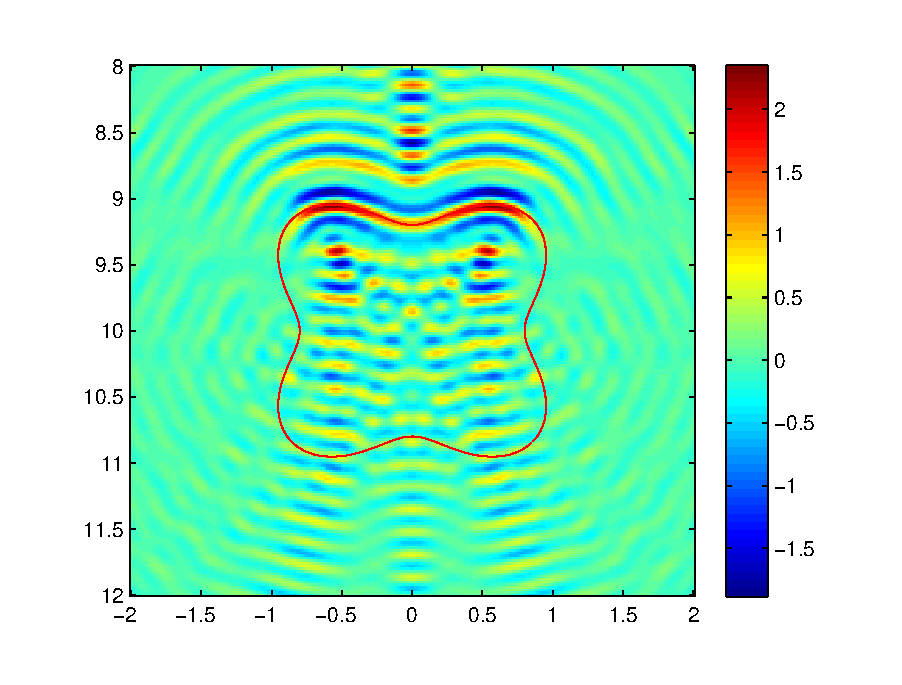
\includegraphics[width=0.32\textwidth]{./graphic/p_leaf_3pi.eps}
	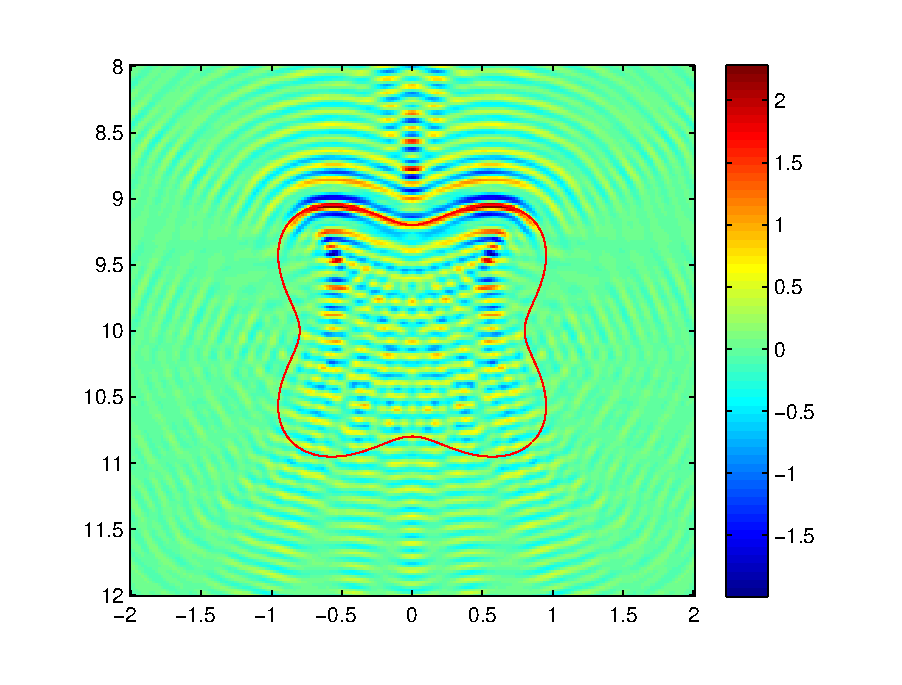
\includegraphics[width=0.32\textwidth]{./graphic/p_leaf_5pi.eps}
	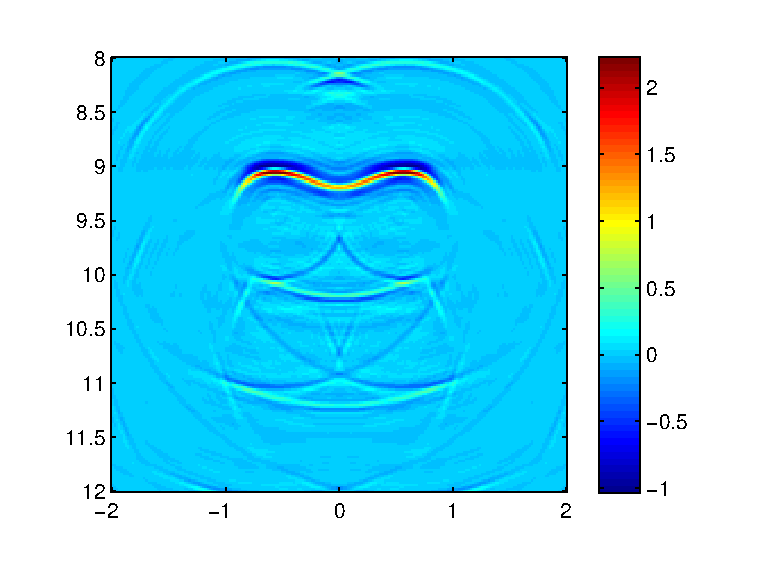
\includegraphics[width=0.32\textwidth]{./graphic/p_leaf.eps}
	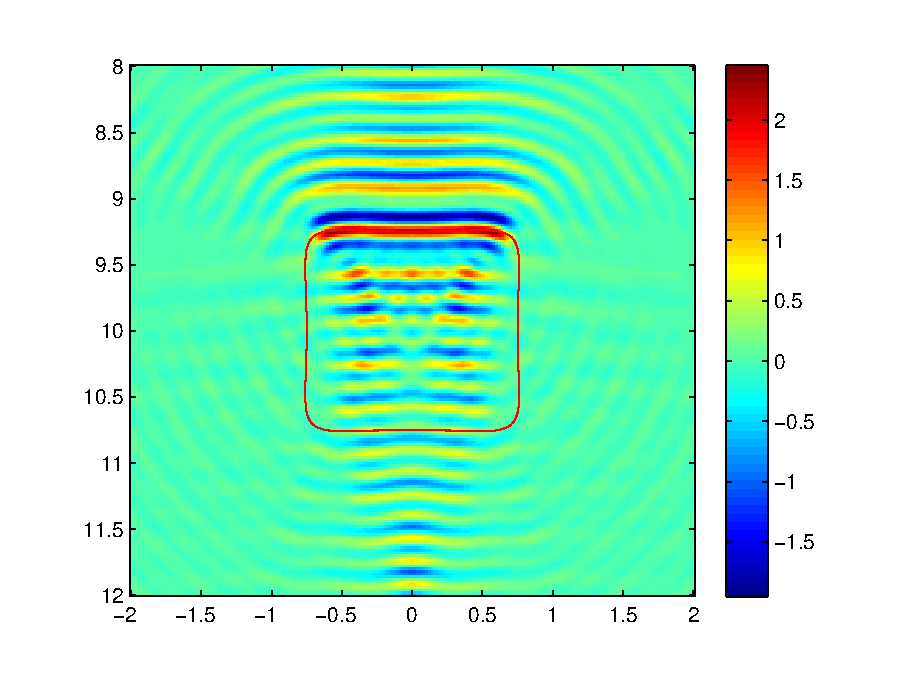
\includegraphics[width=0.32\textwidth]{./graphic/rectangle_3pi.eps}
	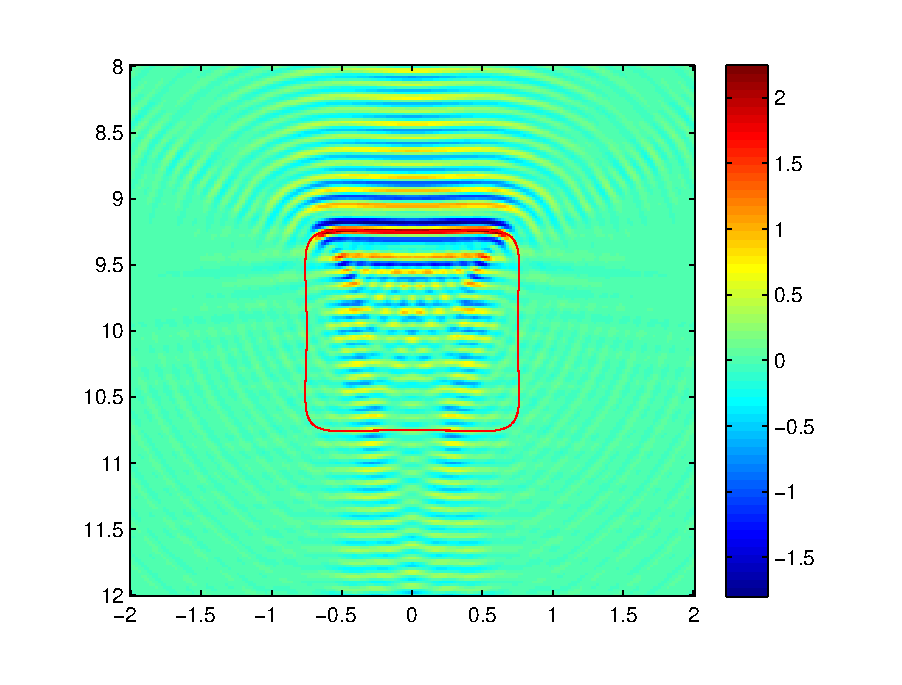
\includegraphics[width=0.32\textwidth]{./graphic/rectangle_5pi.eps}
	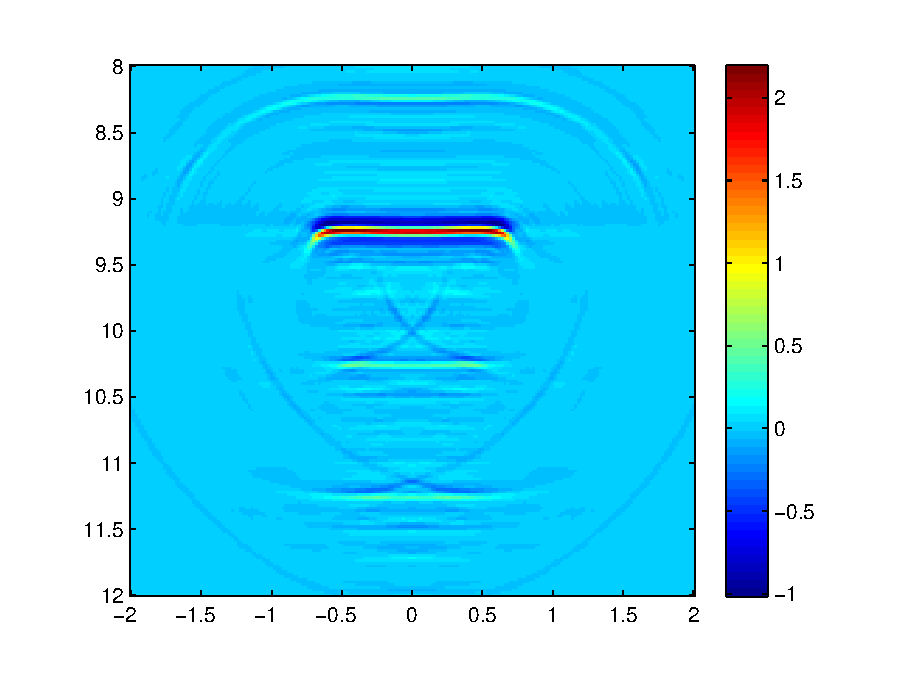
\includegraphics[width=0.32\textwidth]{./graphic/rectangle.eps}
	\caption{算例 1: 从上到下是不同形状的 Dirichlet 障碍物,依次是圆形,花生形,四叶草形 以及旋转后的方形的成像结果. 其中,第一列是关于单频的, 其角频率为 $\om=3\pi$, 第二列是关于单频的, 其角频率为 $\om=5\pi$ 以及第三列是关于多频叠加的.}
	\label{fig_wgout_ex2}
\end{figure}
\end{frame}
\begin{frame}
\frametitle{不同边界条件的障碍物成像}
 \begin{figure}
 \centering
 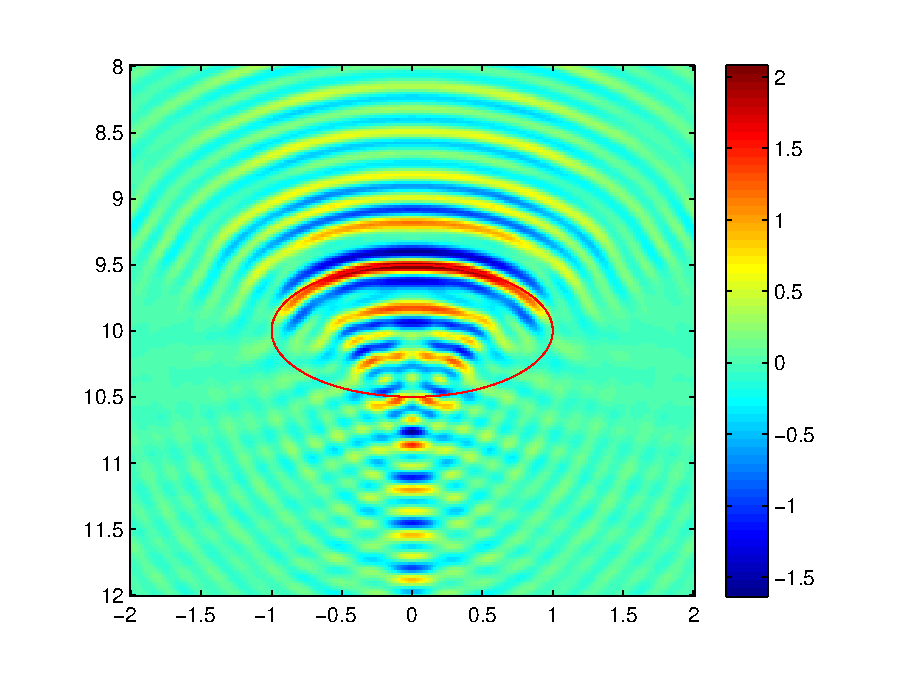
\includegraphics[width=0.24\textwidth]{./graphic/circle_3pi.eps}
 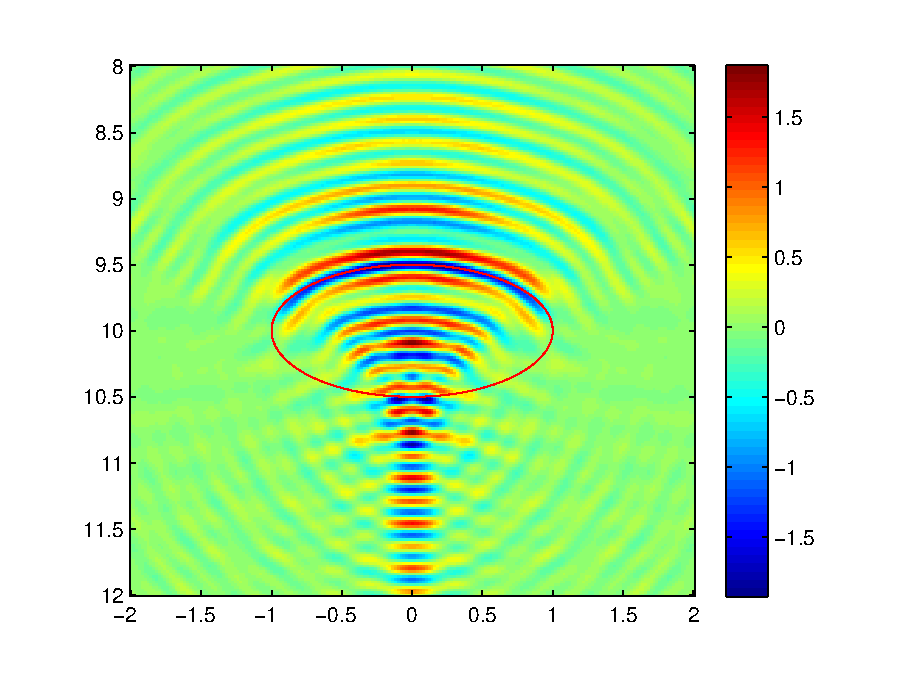
\includegraphics[width=0.24\textwidth]{./graphic/circle_3pi_neumann.eps}
 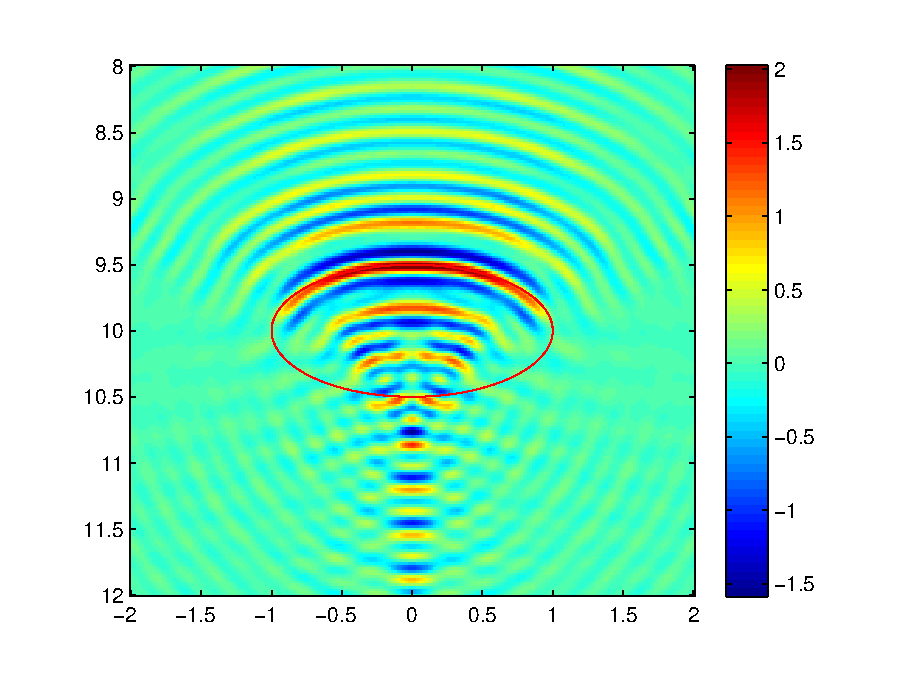
\includegraphics[width=0.24\textwidth]{./graphic/circle_3pi_impedance_1.eps}
 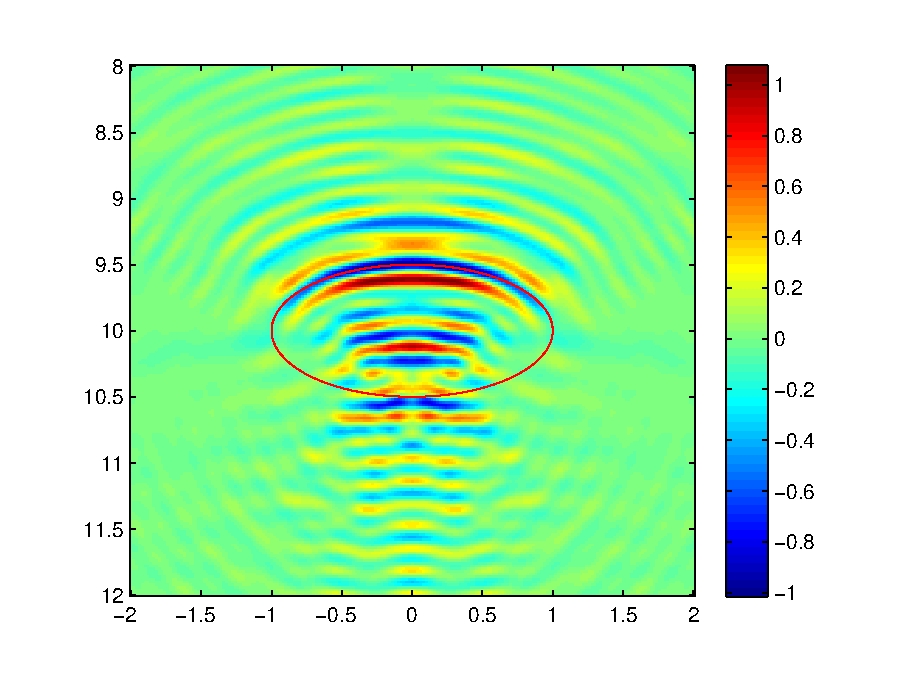
\includegraphics[width=0.24\textwidth]{./graphic/circle_3pi_transmission.eps}
 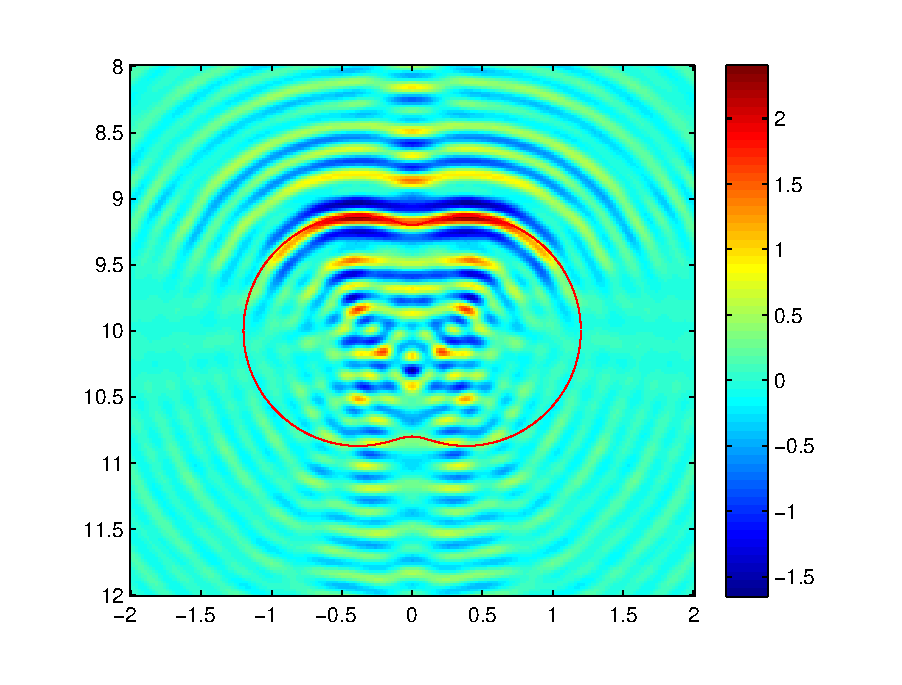
\includegraphics[width=0.24\textwidth]{./graphic/peanut_3pi.eps}
 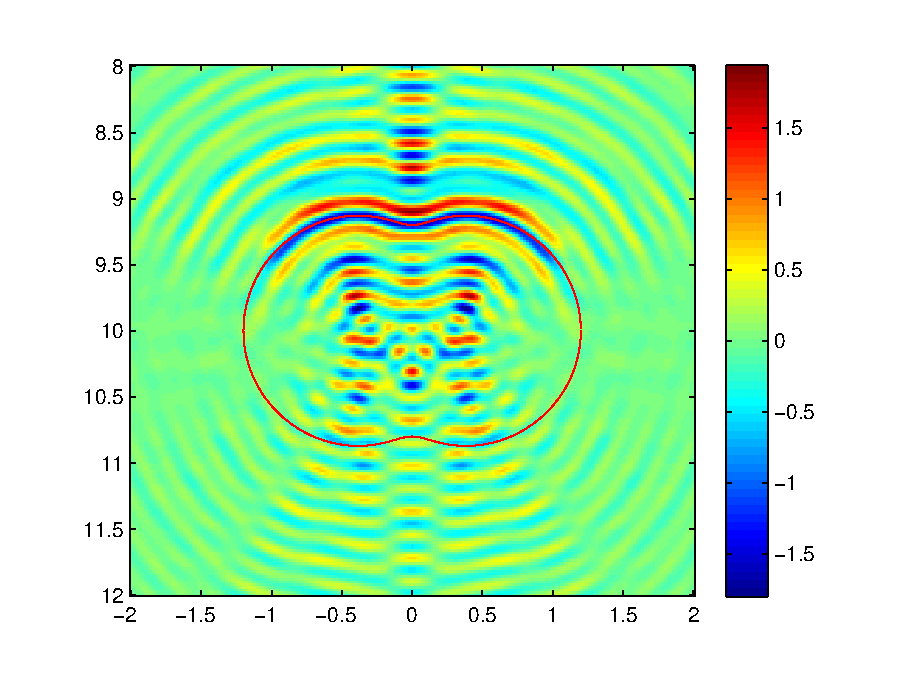
\includegraphics[width=0.24\textwidth]{./graphic/peanut_3pi_neumann.eps}
 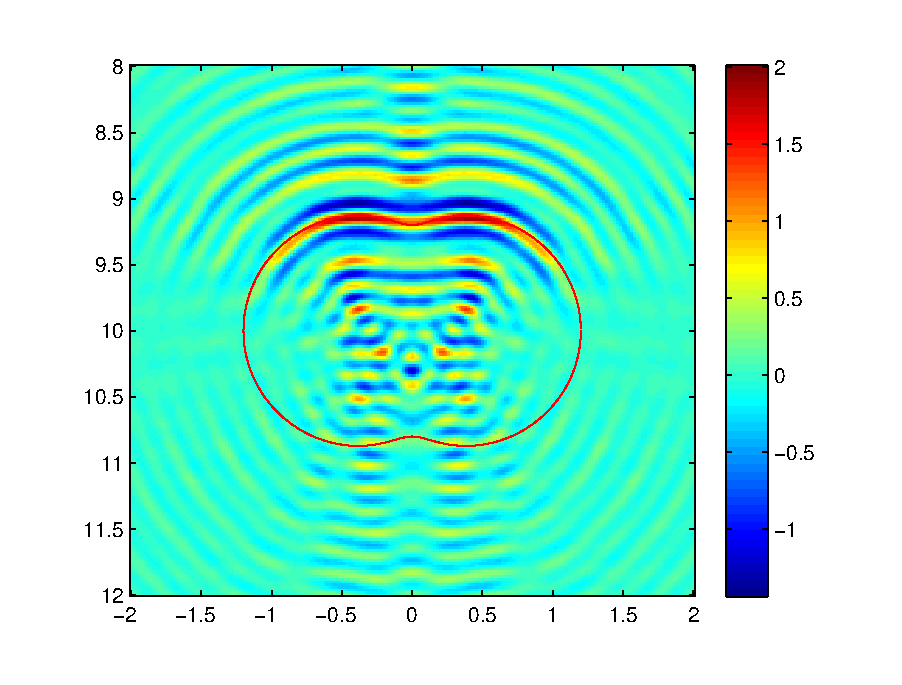
\includegraphics[width=0.24\textwidth]{./graphic/peanut_3pi_impedance_1.eps}
 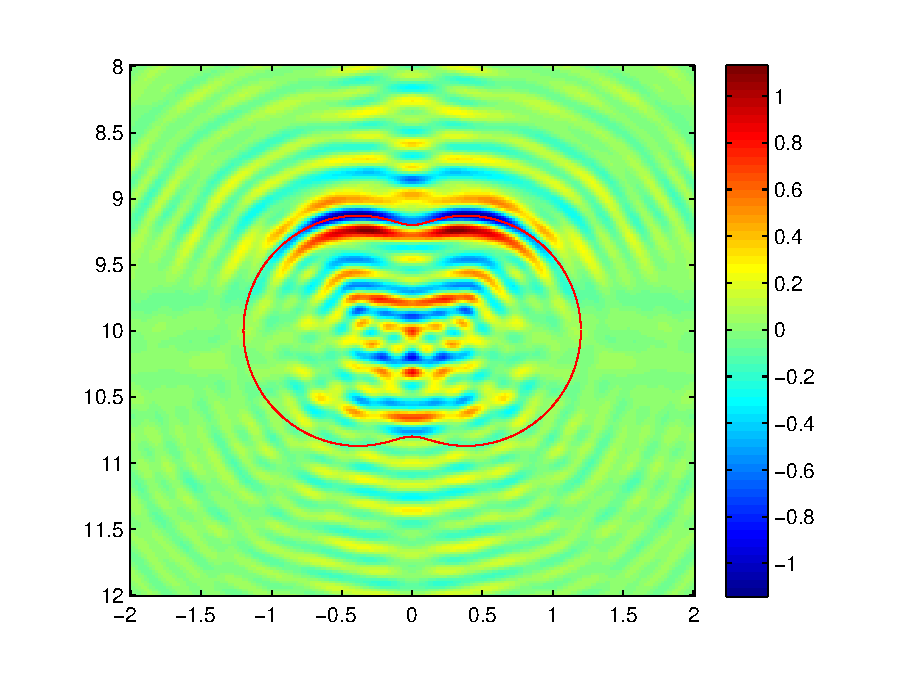
\includegraphics[width=0.24\textwidth]{./graphic/peanut_3pi_transmission.eps}
 \caption{算例 2: 从左到右: Neumann 障碍物, 阻抗障碍物, 以及衍射指数为$n(x)=0.25$ 可穿透障碍物的成像结果 ; 第一行中的障碍物为圆形,第二行中的障碍物为花生.}
 \end{figure}
\end{frame}


\begin{frame}
\frametitle{针对两个障碍物成像:平行情形}
\begin{figure}[h]
	
		\centering
	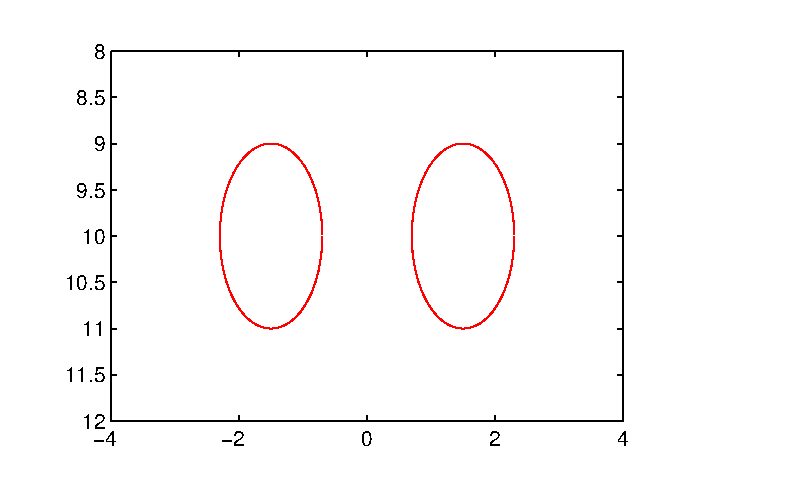
\includegraphics[width=0.32\textwidth,height=0.33\textheight]{./graphic/bi_circle_profile.eps}
	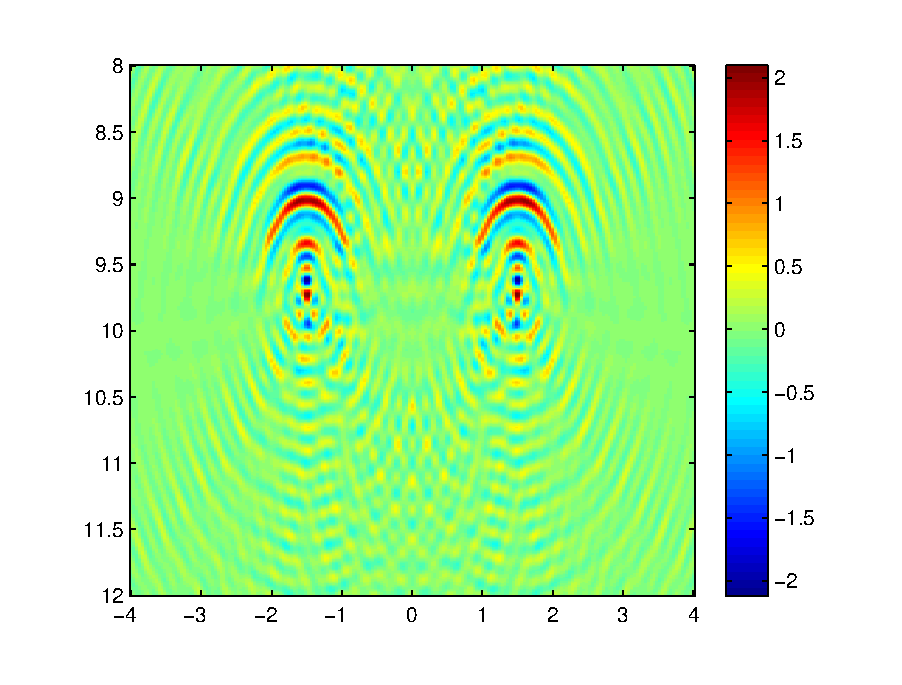
\includegraphics[width=0.32\textwidth]{./graphic/bi_circle_3pi.eps}
	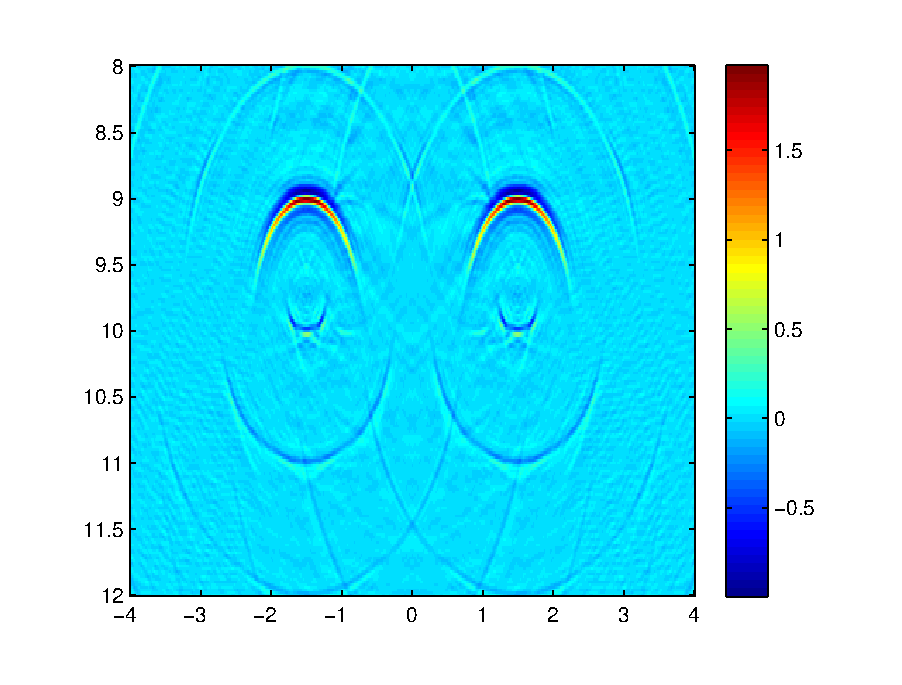
\includegraphics[width=0.32\textwidth]{./graphic/bi_circle.eps}
	
	\caption{算例 3: 从左到右分别为,  真实的两个障碍物:圆, 关于单频角频率为 $\om=3\pi$的成像结果, 关于多频叠加的成像结果.}
\end{figure}
\end{frame}

\begin{frame}
\frametitle{针对两个障碍物成像:上小下大}
\begin{figure}[h]
	
	\centering
	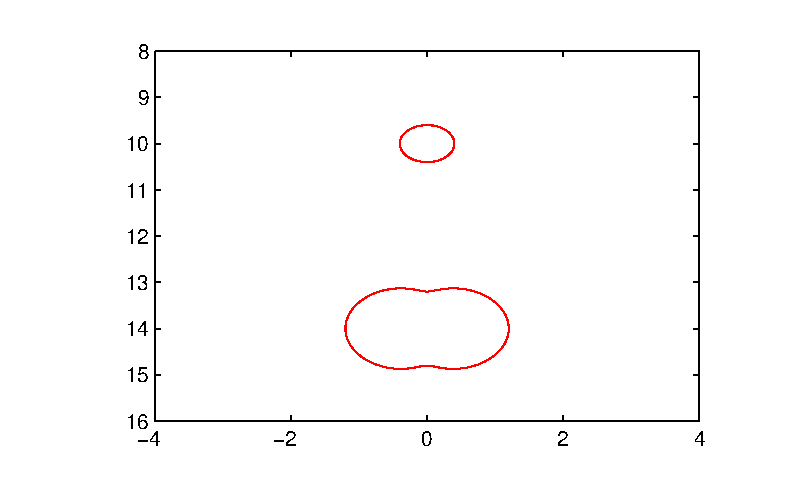
\includegraphics[width=0.32\textwidth,height=0.33\textheight]{./graphic/circle_0_4_peanut_1_profile.eps}
	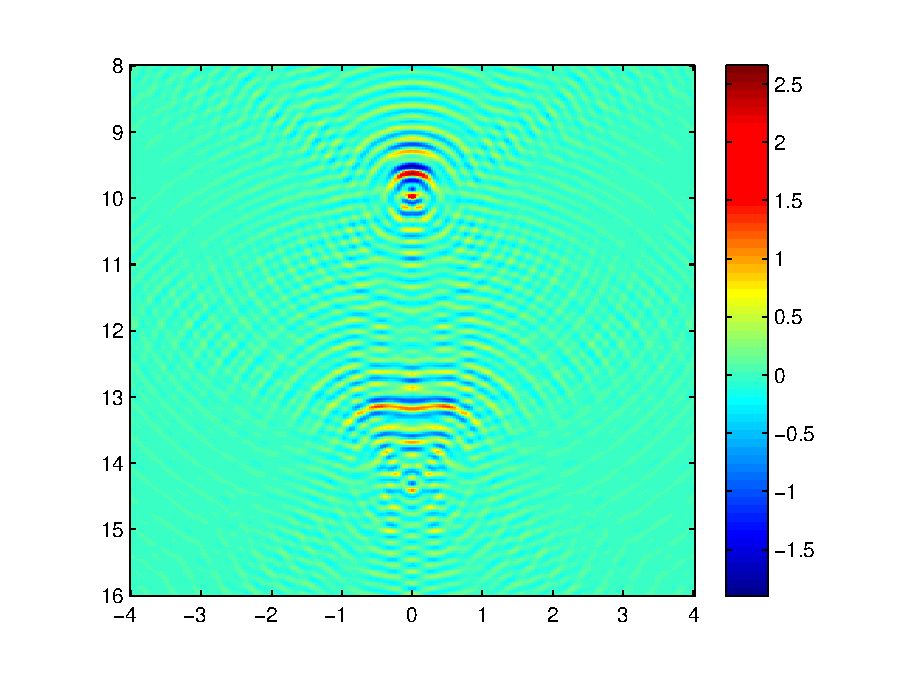
\includegraphics[width=0.32\textwidth]{./graphic/circle_0_4_peanut_1_3pi_1.eps}
	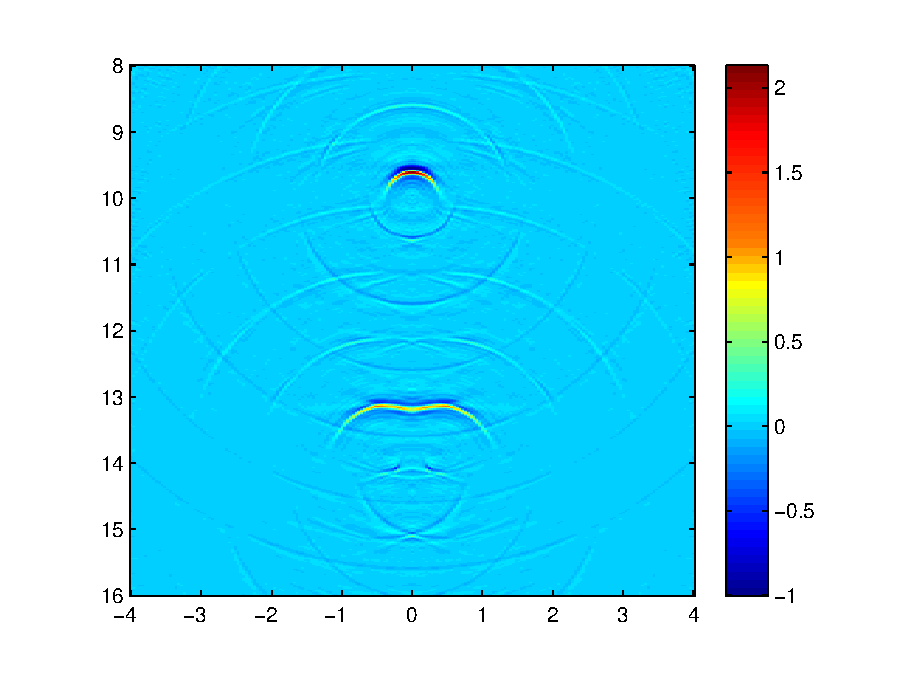
\includegraphics[width=0.32\textwidth]{./graphic/circle_0_4_peanut_1_multi_1.eps}
	
	\caption{算例 3: 从左到右分别为,  真实的两个障碍物:圆上和花生下, 关于单频角频率为 $\om=3\pi$的成像结果, 关于多频叠加的成像结果.}
\end{figure}
\end{frame}

\begin{frame}
\frametitle{针对两个障碍物成像:上大下小}
\begin{figure}[h]
	
		\centering
	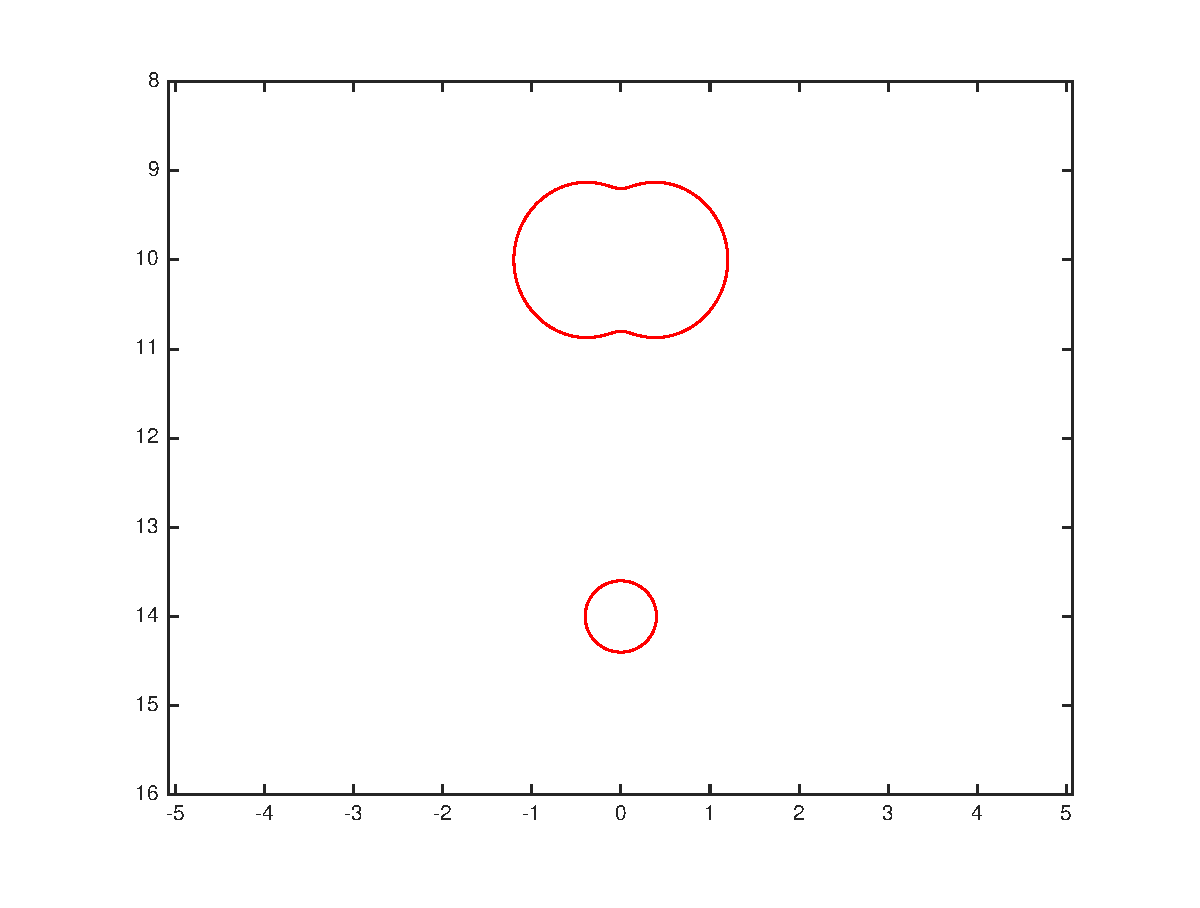
\includegraphics[width=0.32\textwidth,height=0.33\textheight]{./graphic/circle_0_4_peanut_1_profile_reverse.eps}
	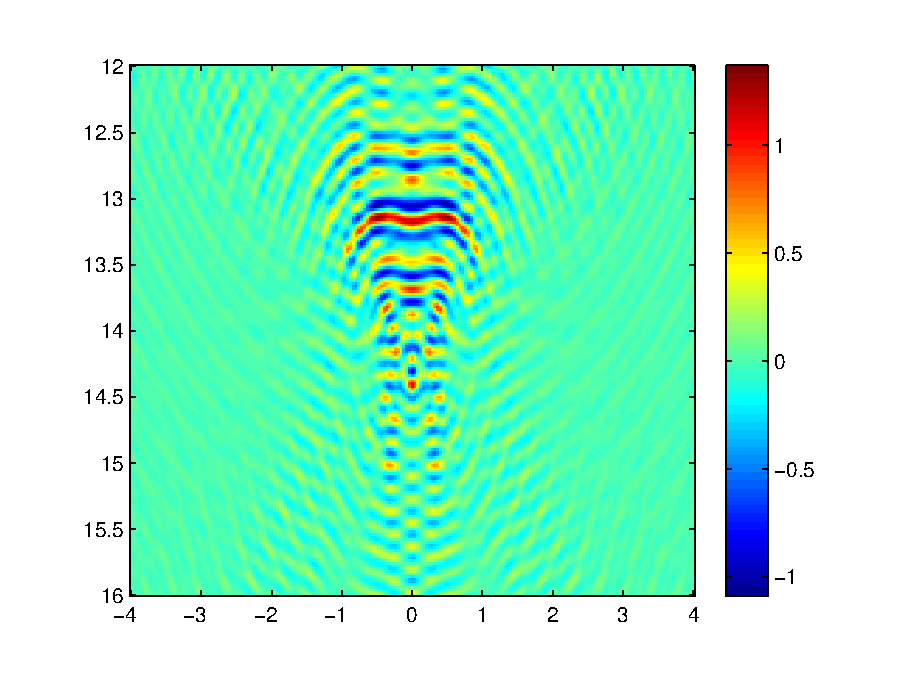
\includegraphics[width=0.32\textwidth]{./graphic/circle_0_4_peanut_1_3pi_down.eps}
	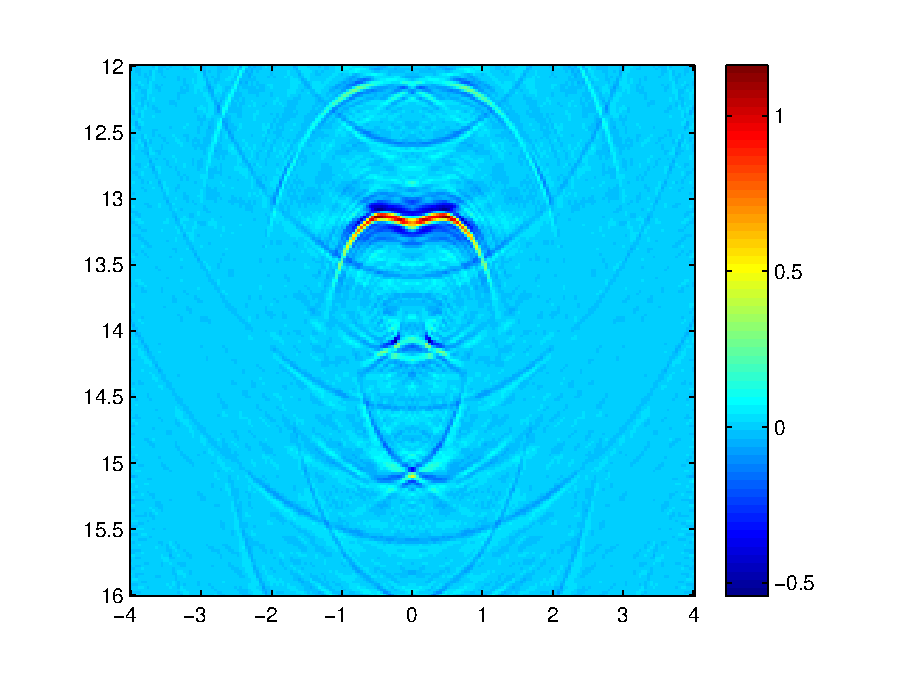
\includegraphics[width=0.32\textwidth]{./graphic/circle_0_4_peanut_1_multi_down.eps}
	
	\caption{算例 3: 从左到右分别为,  真实的两个障碍物:圆下和花生上, 关于单频角频率为 $\om=3\pi$的成像结果, 关于多频叠加的成像结果.}
\end{figure}
\end{frame}

\begin{frame}
\frametitle{观测数据带加性 Gaussian 噪声的成像}
\begin{figure}[h]
	\centering
	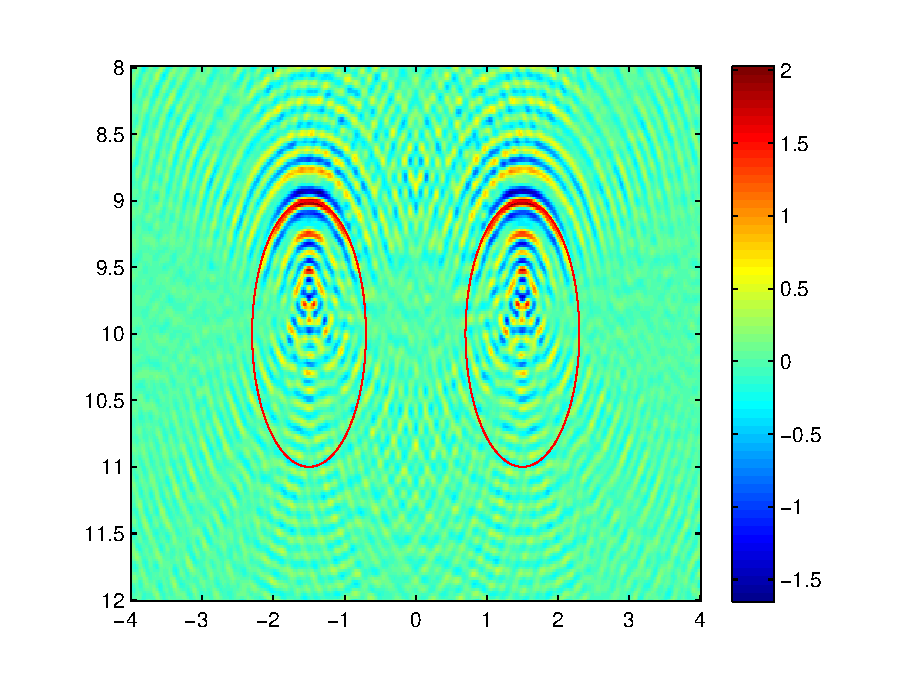
\includegraphics[width=0.32\textwidth]{./graphic/bi_circle_4pi_error2.eps}
	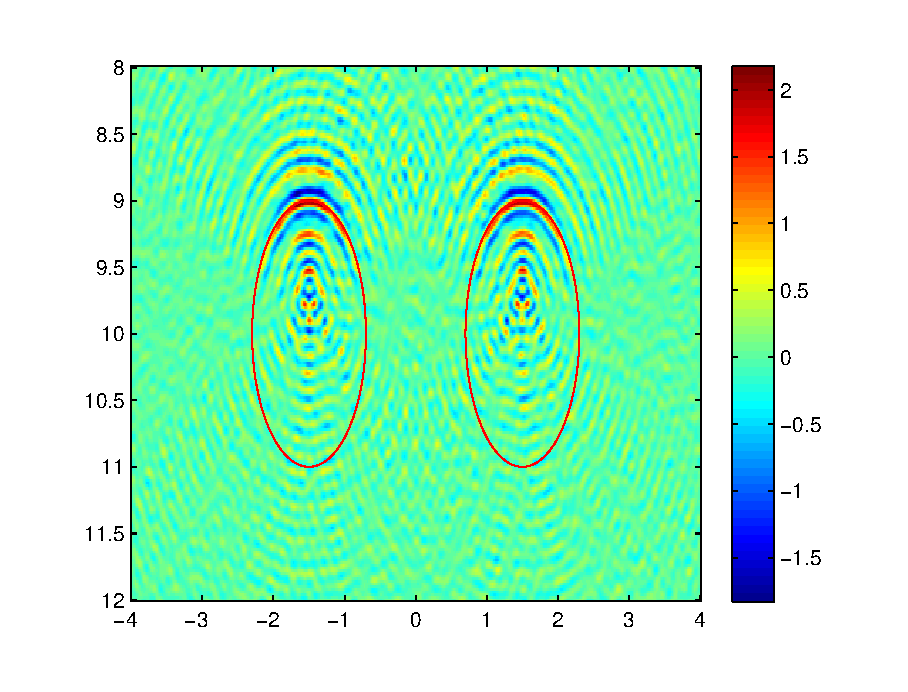
\includegraphics[width=0.32\textwidth]{./graphic/bi_circle_4pi_error4.eps}
	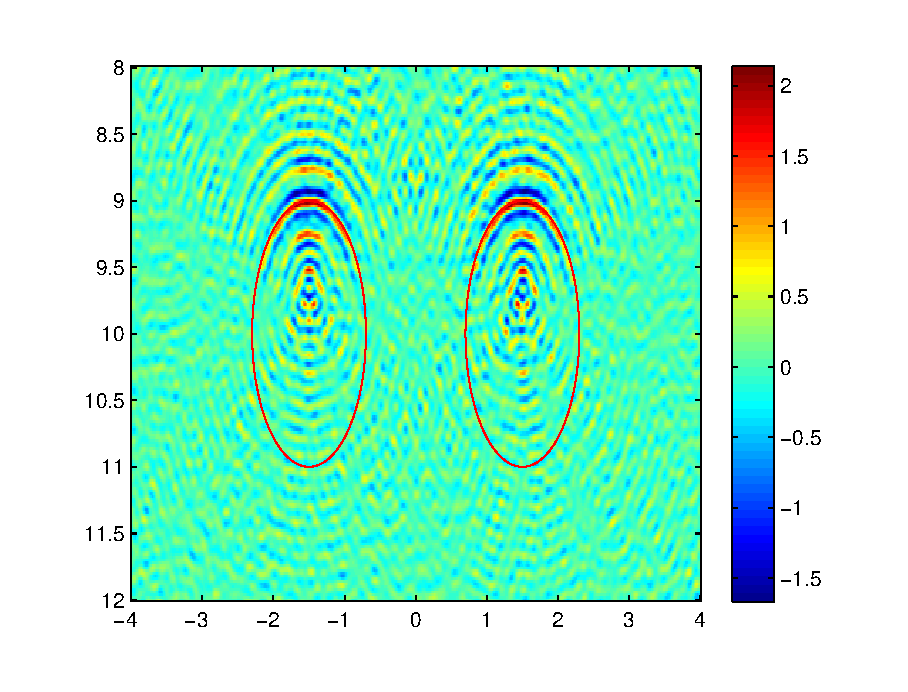
\includegraphics[width=0.32\textwidth]{./graphic/bi_circle_4pi_error6.eps}
	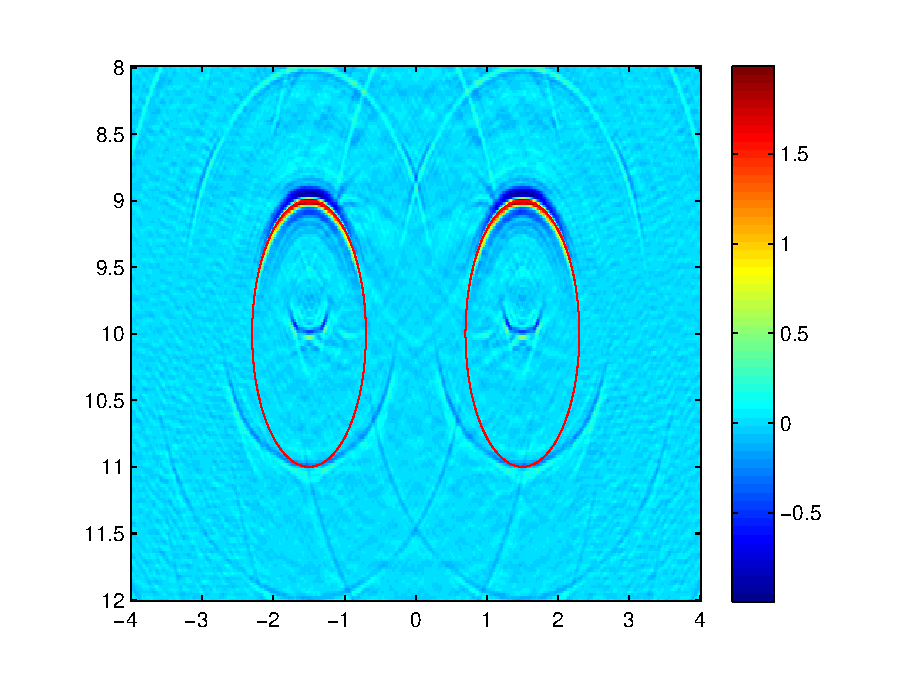
\includegraphics[width=0.32\textwidth]{./graphic/bi_circle_multi_2_8_error2.eps}
	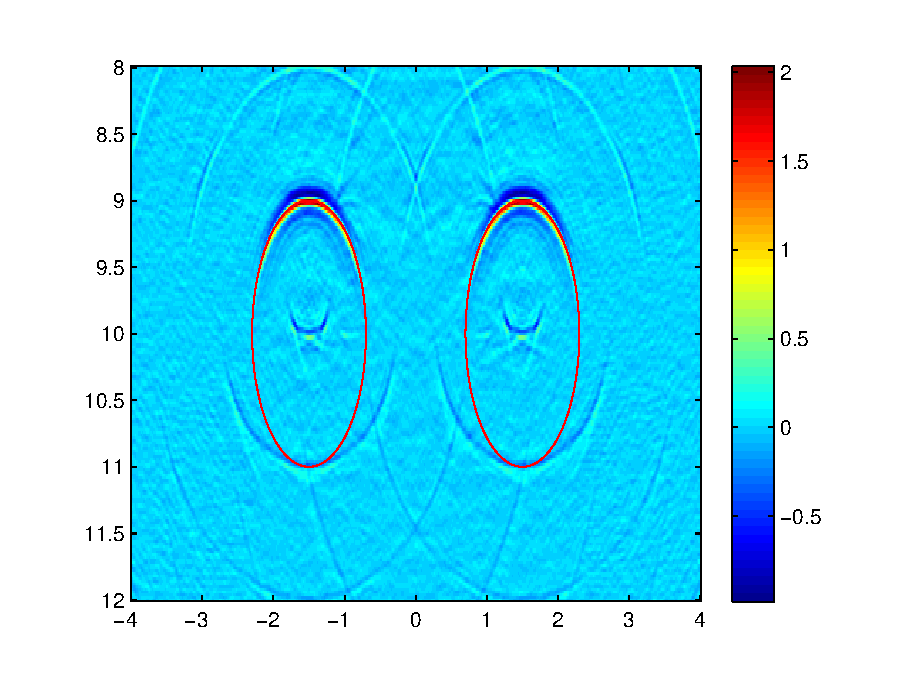
\includegraphics[width=0.32\textwidth]{./graphic/bi_circle_multi_2_8_error4.eps}
	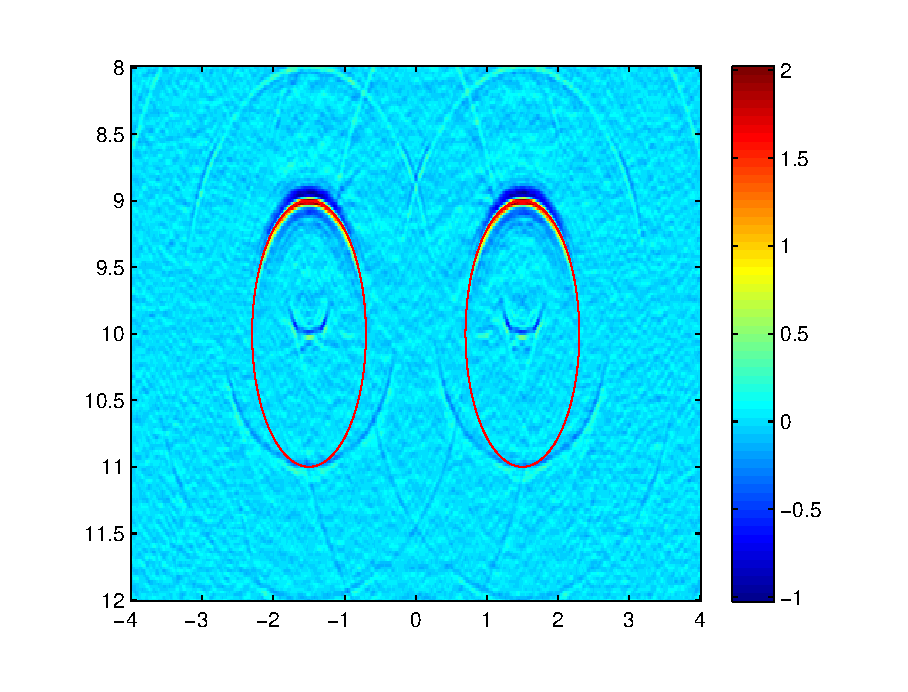
\includegraphics[width=0.32\textwidth]{./graphic/bi_circle_multi_2_8_error6.eps}
	
	\caption{算例 4: 从左到右,分别是含有噪声水平 $\mu =  0.2; 0.3; 0.4$ Dirichlet 障碍物的成像结果. 其中第一行是关于单频成像, 其角频率为 $\om=4\pi$, 第二行是多个单频成像的叠加.}
\end{figure}
\end{frame}

\section{总结与展望}
\begin{frame}
\frametitle{总结}
\begin{itemize}
\item 利用 Fourier 变换推导出了两种半空间 Green 函数: Neumann Green 函数和 Dirichlet Green 函数. 通过研究振荡积分的衰减性质,给出了当 $x\in \Ga_0, \ y\in \R^2_+$ 时, $\N(x,y)$ 和 $\T_D(x,y)$ 随着 $x_2$ 增大的衰减估计.该估计也保证了点扩散函数的定义有意义.
\vspace{.25cm}
\item 针对点源成像问题,给出了点扩散函数.给出来PSF与有限孔径PSF之间的关于孔径 $d$ 的误差估计.利用极限吸收原理及 Fourier 分析找到了 $\J(z,y)$ 的主项$\F(z,y)$,并且刻画了$\J(z,y)-\F(z,y)$关于 $h$ 的衰减估计. 证明了 $\F(z,y)$ 与弹性波基本解 $\G(z,y)$ 有相似的函数性质.
\vspace{0.25cm}
\item 基于点扩散函数, 我们针对基于逆时偏移的直接成像法给出了严格的数学刻画: 其成像函数在远离散射体边界的时候快速衰减. 而且,该分辨率分析不需要高频渐近假设或几何光学近似,对一般的边界条件都成立. 利用 kirchhoff 逼近说明了成像函数只在散射体面向接收面的那部分形成较大的峰值.
\end{itemize}
\end{frame}
\begin{frame}
\frametitle{展望}
\begin{itemize}
	\item 由于半空间的Green 函数都是以震荡积分的形式表述,当频率较大时, 我们需要快速算法来计算. 其中,可否将 Green 函数进行渐近级数展开是一个有趣的问题.本文针对 Green 函数衰减性的研究局限在 $\Ga_0$ 上,将来如果可以将研究范围延拓到半空间上甚至是复数域上, 将有助于对半空间弹性波散射问题的 PML 方法的研究.
	\vspace{.25cm}
	\item 关于发展接收数据不是全波位移数据的算法.
	在实际问题中, 数据的相位可能不好获取,由于弹性波数据中横波数据和纵波数据耦合在一起, 所以当只接收到混合波的振幅数据时, 很难效仿针对声波,电磁波的算法来构造成像函数. 进一步,针对真实的勘探模型, 一般 $e_2$ 方向的位移数据更容易得到, 于是如何只用接收到的数据 $u^s_q(x_r,x_s)\cdot e_2, \ q=e_1, \ e_2$ 甚至仅用 $u^s_{e_2}(x_r,x_s)\cdot e_2$ 去成像也是个有意义的研究问题.
\end{itemize}
\end{frame}

\begin{frame}
	\vspace{1cm}
	\centerline{\Huge \textcolor{red}{谢谢大家!}}
\end{frame}
\end{document}

